\chapter{Methods}

In the previous section we talked about the background and demand for sentiment analysis system, the history of research, the general goal and challenges in this area, and some specific tasks for the researchers to work on. In this section, we will introduce some methods used for solving some of the tasks defined above; specifically, we will put most of our attention to statistical and machine learning methods, because of their generalization ability - one method can often be applied to many similar tasks with similar formulations without us having to look at the data and hand-craft features.

We will start with some important features; then we will talk about topic modeling methods that are widely used in factual information analysis, and their variations designed specifically for sentiment analysis problems; finally we will talk about the deep learning methods for natural language processing. In the past several years, we witnessed the ``tsunami" of deep learning in many fields, especially in computer vision and speech recognition. We will briefly introduce the history of deep learning, with an emphasis of its application in natural language processing, and then introduce several important models including word embedding, neural network language model and recurrent neural network, which are used in our framework.

\section{Features}

In the data-driven approaches for natural language processing, we often convert a piece of text into a feature vector that the statistical models can process. A large volume of work is devoted to the feature selection problem of machine learning. However, the discussion of such techniques is out of the scope of this paper. Instead, we will focus on some important features and related methods specific to sentiment analysis.

\subsection{Term Presense and Frequency}

In information retrieval, it is traditional to represent a text as a feature vector where each entry of the vector corresponds to the number of appearances of some specific term in the text. This frequency-based fashion is popular in information retrieval, seen in examples like the widely used tf-idf weighting. However, it is reported in \cite{pang2002thumbs} that in polarity classification, a better performance can be obtained using presence instead of frequency. Using presence means that each entry of the feature vector merely indicates whether a term appeared or not in the text. This observation shed light on the difference of topic-based and sentiment-based problems: while a topic is more likely to be emphsized by the frequent appearances of certain words, sentiment might not be strengthened by such repetition. 

One natural extention to single term frequency is higher-order n-grams. The effectiveness of using n-grams is yet to be discussed. \cite{pang2002thumbs} reported that higher performance can be achieved with unigrams than bigrams when classifying movie reviews by sentiment polarity, whilc \cite{dave2003mining} reported that in some settings bigrams can trigrams can outperfom unigrams in product review polarity classification.

\subsection{Part-of-speech}

One of the reasons that part-of-speech information's wide use in not just sentiment analysis but general text analysis is: part-of-speech tagging is a crude form of word sense disambiguation. One of the earliest use of data-driven approach for the prediction of semantic orientation of words was developed for adjectives. Subsequent work on subjectivity detection demonstrated a high correlation between the use of adjectives and subjectivity \cite{hatzivassiloglou2000effects}. This observation has often been seen as an evidence that certain adjectives are good indicators of sentiment. In extention to just using adjectives, \cite{turney2002thumbs} proposed to use a number of pre-defined part-of-speech pattern to select phrases (most contain adjectives or adverbs), which is later used to detect document sentiment. Beside adjectives, verbs and nouns can also be used for expressing sentiment; as reported in \cite{pang2002thumbs}, using only adjectives as features lead to much worse performance than using the same number of most frequent unigrams. 
% For sentiment analysis, adjectives have been used as important features in a number of works \cite{mullen2004sentiment,whitelaw2005using}. 

\subsection{Negations}

Negations is a key factor in the expression of sentiment, because a single negation can completely reverse the sentiment polarity. Despite of the semantic importance, negations are not specifically treated in term-based vector representations. This is not much of a problem in information retrieval since a negation cannot drastically change the topic of a piece of text. However, this is problematic for sentiment analysis, especially when there is double negation. It is possible to deal with negations indirectly using second-order features, that is, for example \cite{das2001yahoo} proposed to attach ``NOT" to words occuring close to negation terms. This can be extended to a more subtle and accurate method by using at the parsing tree. In \cite{na2004effectiveness}, the authors looked for specific part-of-speech tag patterns for negations, and tag the complete phrase as a negation phrase. Further improvement is achieved by using deeper analysis of the syntax \cite{kennedy2006sentiment}.

\section{Topic Modeling Methods}

Topic modeling is a method for analyzing large quantities of unlabeled data - it's an unsupervised method. For the purpose of sentiment analysis, or more generally text analysis, a topic is a probability distribution over a collection of words. A topic model is generative model that describes the procedure of the generation of the topics, defined by the statistical relationship between a group of observed and latent random variables. The goal of having the topics is to provide a thematic summary of a collection of documents - they tell us about the themes of those documents. For example a collection of news articles might have themes of politics, business, culture, and science.

\subsection{Latent Dirichlet Allocation}

Latent Dirichlet Allocation (LDA) \cite{blei2003latent} is arguably the most popular topic model in application; it is also very simple. At a high level viewpoint, LDA provides a model that describes the generation process of each document in a collection. The collection of documents is denoted as $D$, and the vocabulary set is denoted as $V$. LDA requires a constant $K$ - the number of topics, it needs to be defined beforehand.
Each topic $i$ of LDA is model by a multinomial distribution $\beta_i$ of all the  words in $V$. Each document is modeled as a multinomial distribution $\alpha$ over the $K$ topics. The generation process is:

For each document:
\begin{itemize}
    \item[1.] draw a topic distribution over the $K$ topics, $\theta\sim \text{Dir}(\alpha)$; $\text{Dir}(\alpha)$ is the dirichlet distribution with scaling factor $\alpha$; $\theta$ is a vector of length $K$ denoting the probability of each topic;
    \item[2.] for each word $w_n$ in the document:
        \begin{itemize}
            \item[i.] draw a topic $z_n\sim \text{Mult}(\theta)$ from the $K$ topics; $\text{Mult}(\theta)$ is a multinomial distribution defined by $\theta$;
            \item[ii.] draw a word $w_n\sim \beta_{z_n}$.
        \end{itemize}
\end{itemize}

Note that $\alpha$ is actually $(\alpha_1, \alpha_2, ..., \alpha_K)$, $K$ parameters for the dirichlet distribution.
We use a one-hot vector $w$ to represent a word, and if the integer index of thw word in the dictionary is $u$, then $w^u=1$ and $w^v=0$ for all $v\neq u$. We use $\vw=(w_1, w_2, ..., w_N)$ to denote a document with $N$ words.
We use a one-hot vector $z$ to represent the selection of topic - the $i$th element of $z$ is 1 if we select the $i$th topic. We use $\vz=(v_1, v_2, ..., v_N)$ to represent the topic selction of the whole document. $\beta$ is a $K\times V$ word-probability matrix for each topic (row) and each word (column), $\beta_{i,j} = p(w^j=1|z^i=1)$

Before diving into the inferential problem of LDA, we emphasize on several characteristics of the LDA model:

\begin{itemize}
    \item the documents in collection $D$ share the same set of topics;
    \item from process 1. we see that LDA allows each document can contain multiple topics
    \item from process 2. we see that LDA treats each document as a bag of words - the order of the words is ignored;
    \item in LDA, each word is generated from a single topic
    \item topics are allowed to shift quickly - the topic of each word is sampled independently of other words.
\end{itemize}

The inferential problem of LDA is determining the posterior distribution of the latent variables given the observed variables - the documents:

$$p(\theta, \vz | \vw, \alpha, \beta) = \frac{p(\theta, \vz, \vw | \alpha, \beta)}{p(\vw | \alpha, \beta)}$$

We can decompose the numerator into a hierarchy by examing the graphical model:
$$p(\theta, \vz, \vw | \alpha, \beta) = p(\vw | \vz, \beta)p(\vz | \theta)p(\theta| \alpha)$$
As LDA treats the document as a bag of word, $p(\vw | \vz, \beta) = \prod_{n=1}^N \beta_{z_n, w_n}$. Also $p(\vz | \theta)$ is trivial and we can write $p(z_n | \theta)=\theta_i$ such that $z_n^i=1$. Finally, $p(\theta | \alpha)$ is given by:

$$p(\theta | \alpha) = \frac{\Gamma(\sum_{i=1}^K \alpha_i)}{\prod_{i=1}^K \Gamma(\alpha_i)} \prod_{i=1}^K \theta_i ^ {\alpha_i - 1}$$

Putting all these together we have the numerator:

$$p(\theta, \vz, \vw | \alpha, \beta) = \left(\frac{\Gamma(\sum_{i=1}^K \alpha_i)}{\prod_{i=1}^K \Gamma(\alpha_i)} \prod_{i=1}^K \theta_i ^ {\alpha_i - 1}\right) 
\prod_{n=1}^N \prod_{i=1}^K \prod_{j=1}^V (\theta_i \beta_{i,j})^{w_n^jz_n^j}$$

To obtain the denominator, we marginalize over $\theta$ and $\vz$:

$$p(\vw | \alpha, \beta) = \frac{\Gamma(\prod_{i=1}^K \alpha_i)}{\prod_{i=1}^K \Gamma(\alpha_i)} \int \left(\prod_{i=1}^K \theta_i^{\alpha_i - 1}\right)
\left(\prod_{n=1}^N \sum_{i=1}^K \prod_{j=1}^V (\theta_i\beta_{i,j})^{w_n^j}\right)
d\theta $$

Computing this distribution is intractable as the coupling between $\theta$ and $\beta$ makes it so that when we compute the log of this function, we are unable to seperate the $\theta$ and $\beta$. While the exact inference is intractable, various approximate inference techniques can be used, including Gibbs sampling and variational inference. However the introduction of inference methods is out of the scope of this paper since we want to focus on the models, so we will not skip it and encourage the readers to refer to \cite{steyvers2005probabilistic,blei2012probabilistic} for more details. 

To use LDA for text analysis, we need to provide a set of documents and the number of topics $K$. LDA will give us two kinds of distributions: $K$ topics shared across the whole collection, each being a distribution over the whole dictionary; for each document a distribution of the topics. 

\subsection{Variations of LDA}

LDA models a simple generation process which fits many scenarios. However, when used for the extraction of aspects for aspect-based sentiment analysis, due to the problem characteristics analyzed in Chapter 2, the performance of LDA is not satisfactory. Many varaitions of LDA have been proposed specifically for sentiment analysis.

Since in evaluative texts like product reviews, there are aspect words and sentiment words, one design factor of topic model is to use one latent variable for both types or to use seperate latent variables. In addition, the model can also be enhanced by modeling the dependency between aspects and ratings. One can also choose to model only the opinion phrases instead of all the words in the document. Here we first review the formal definition of the graphical model of LDA, as shown in Figure~\ref{fig:methods:LDA_1}:

$$p(\vz, \vw, \theta | \alpha, \beta) = p(\theta, \alpha) \prod_{n=1}^N \left[ 
p(z_n| \theta) p(w_n | z_n, \beta)\right]$$

\begin{figure}
\centering
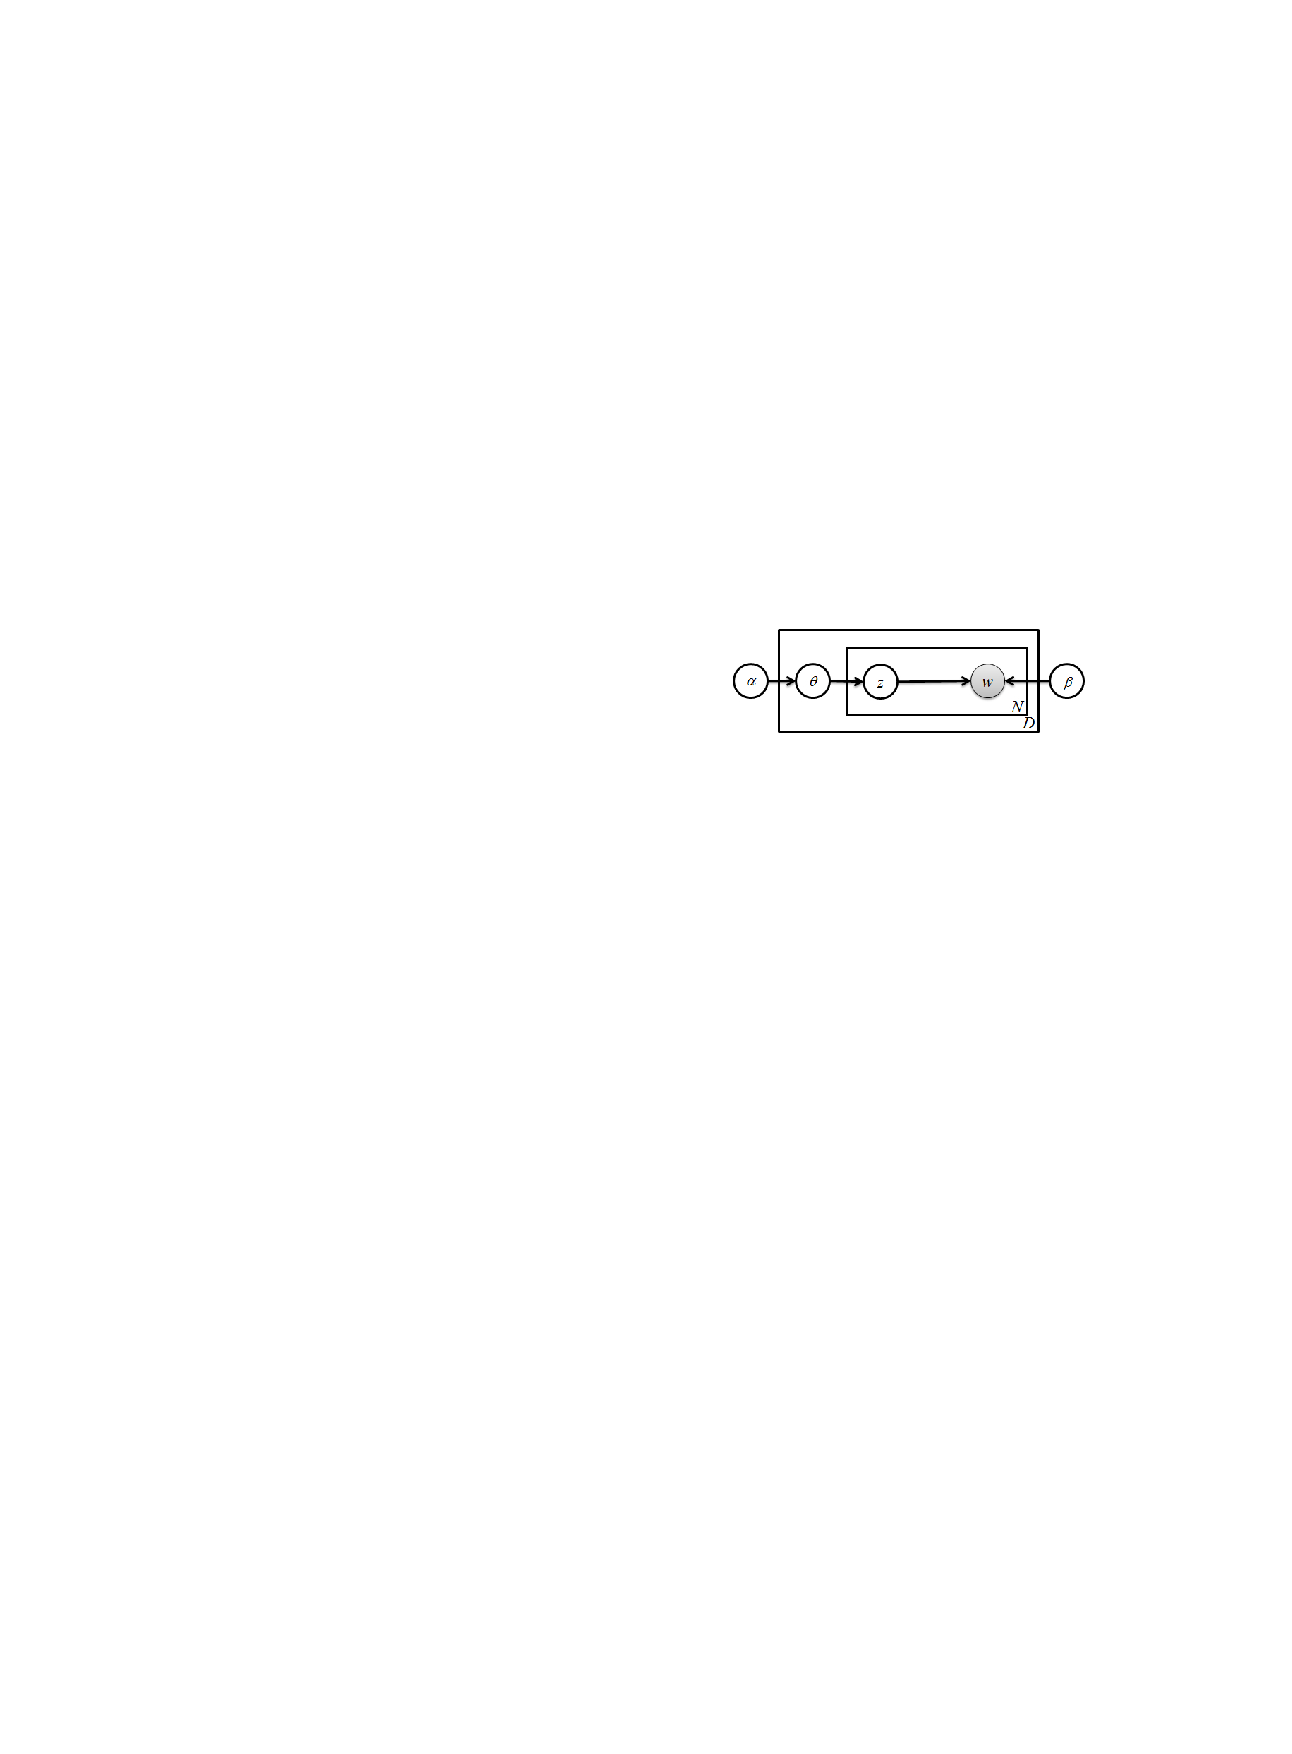
\includegraphics[width=0.5\columnwidth]{figures/methods/LDA_1}
\caption{LDA graphical model. Source of figure: \cite{moghaddam2012design}.}
\label{fig:methods:LDA_1}
\end{figure}

\subsubsection{S-LDA: seperate aspect and rating}

In S-LDA \cite{lakkaraju2011exploiting,moghaddam2012design}, the latent variable for topics $\vz$ is replaced by two seperate variable for aspects and rating respectively. For each aspect-rating pair, $\theta$ contains the probability of generating the corresponding combination. For each review, $\theta$ is sampled once, just like LDA; then $a_n$ and $r_n$ are sampled independently for each word and $w_n$ is sampled conditioned on both latent variable. The formal definition of the generation process is the following, as shown in Figure~\ref{fig:methods:S-LDA}:

$$p(\va, \vr, \vw, \theta | \alpha, \beta) = p(\theta, \alpha) \prod_{n=1}^N \left[ 
p(a_n| \theta) p(r_n | \theta) p(w_n | a_n, r_n, \beta)\right]$$

\begin{figure}
\centering
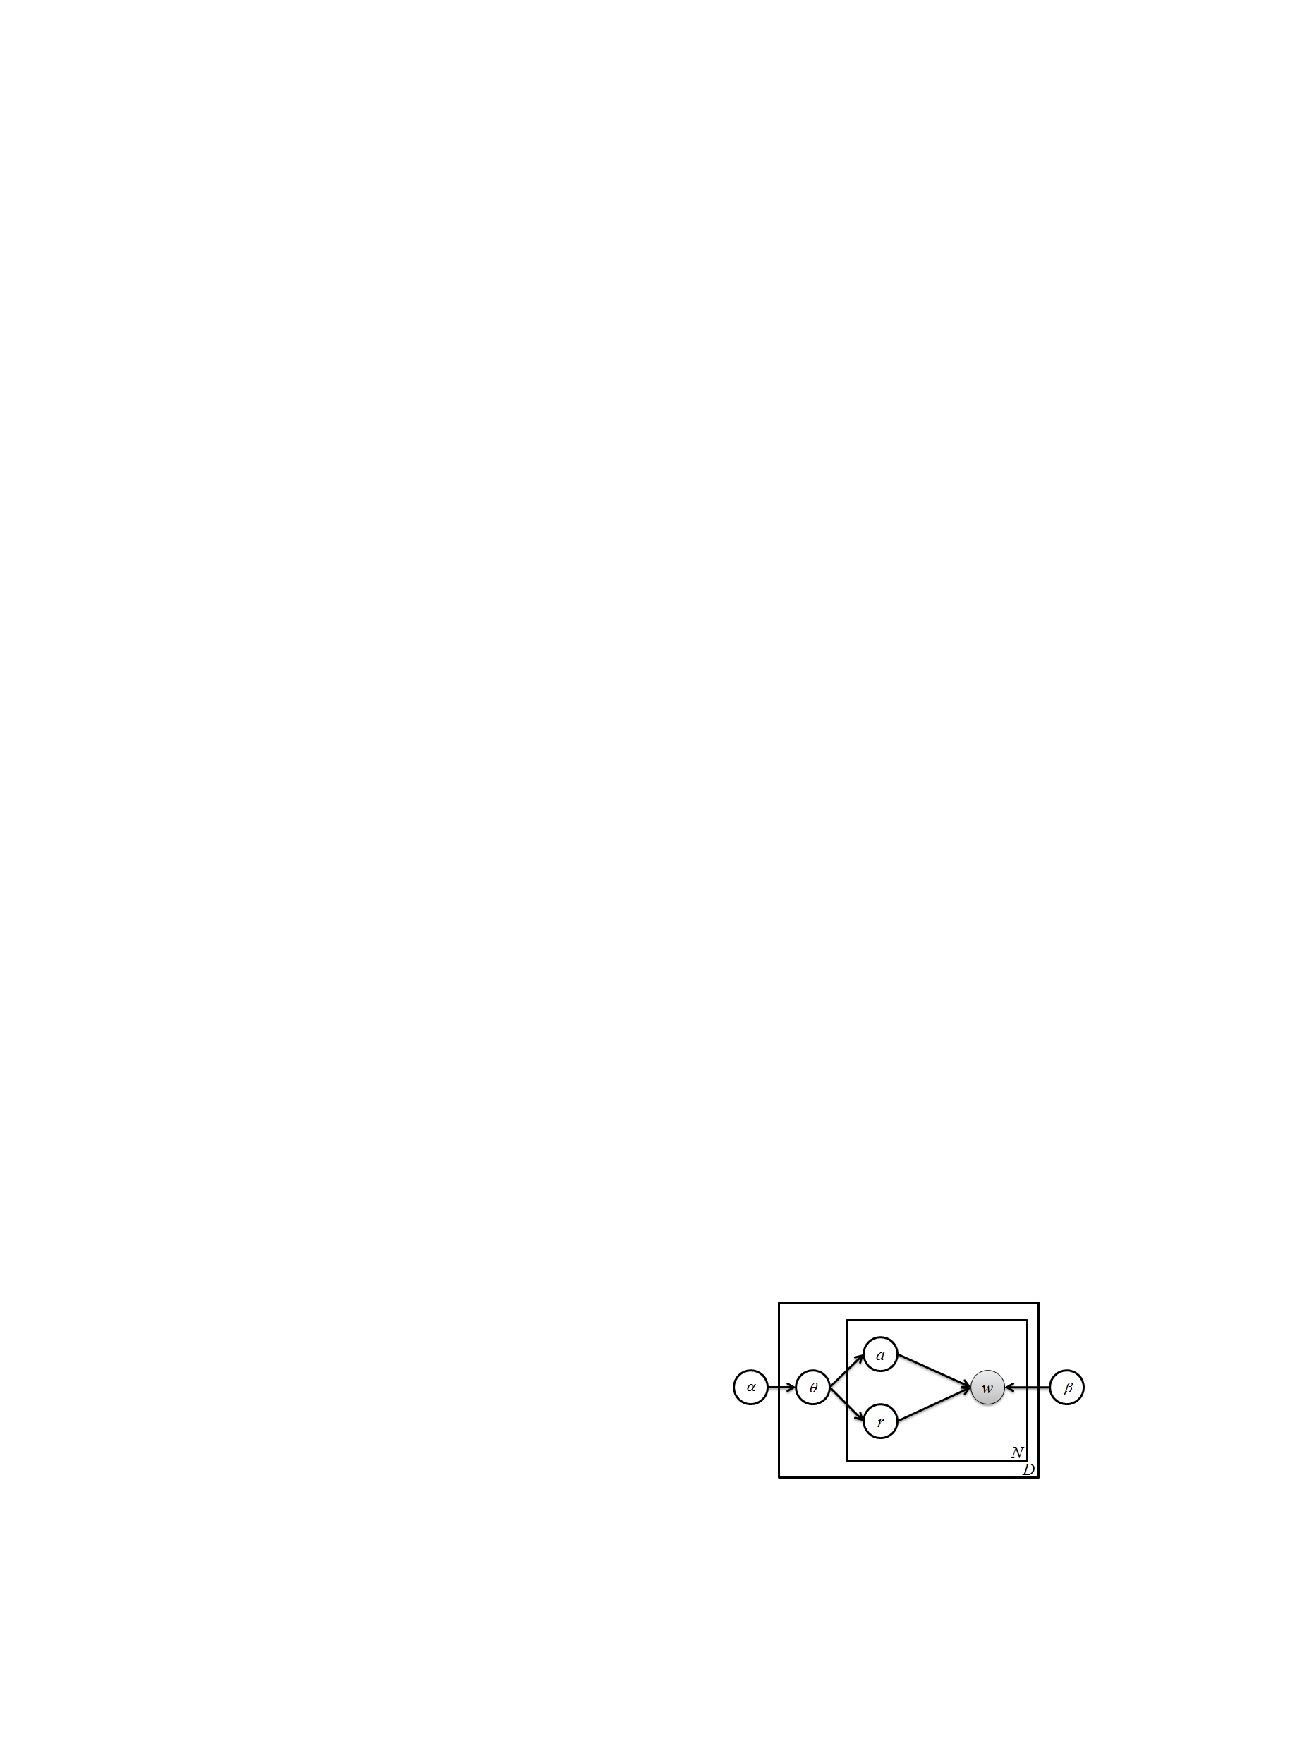
\includegraphics[width=0.5\columnwidth]{figures/methods/S-LDA}
\caption{S-LDA. \cite{moghaddam2012design}}
\label{fig:methods:S-LDA}
\end{figure}

\subsubsection{D-LDA: dependency between aspect and rating}

Several variations of LDA leveraged the dependency between aspects and ratings \cite{he2011automatically,jo2011aspect,li2010sentiment,lin2009joint,moghaddam2011ILDA,moghaddam2012design}.
On the basis of S-LDA, D-LDA further models the dependency of the rating on the aspect. The generation process is the following, as shown in Figure~\ref{fig:methods:D-LDA}:

$$p(\va, \vr, \vw, \theta | \alpha, \beta) = p(\theta, \alpha) \prod_{n=1}^N \left[ 
p(a_n| \theta) p(r_n | a_n, \theta) p(w_n | a_n, r_n, \beta)\right]$$

\begin{figure}
\centering
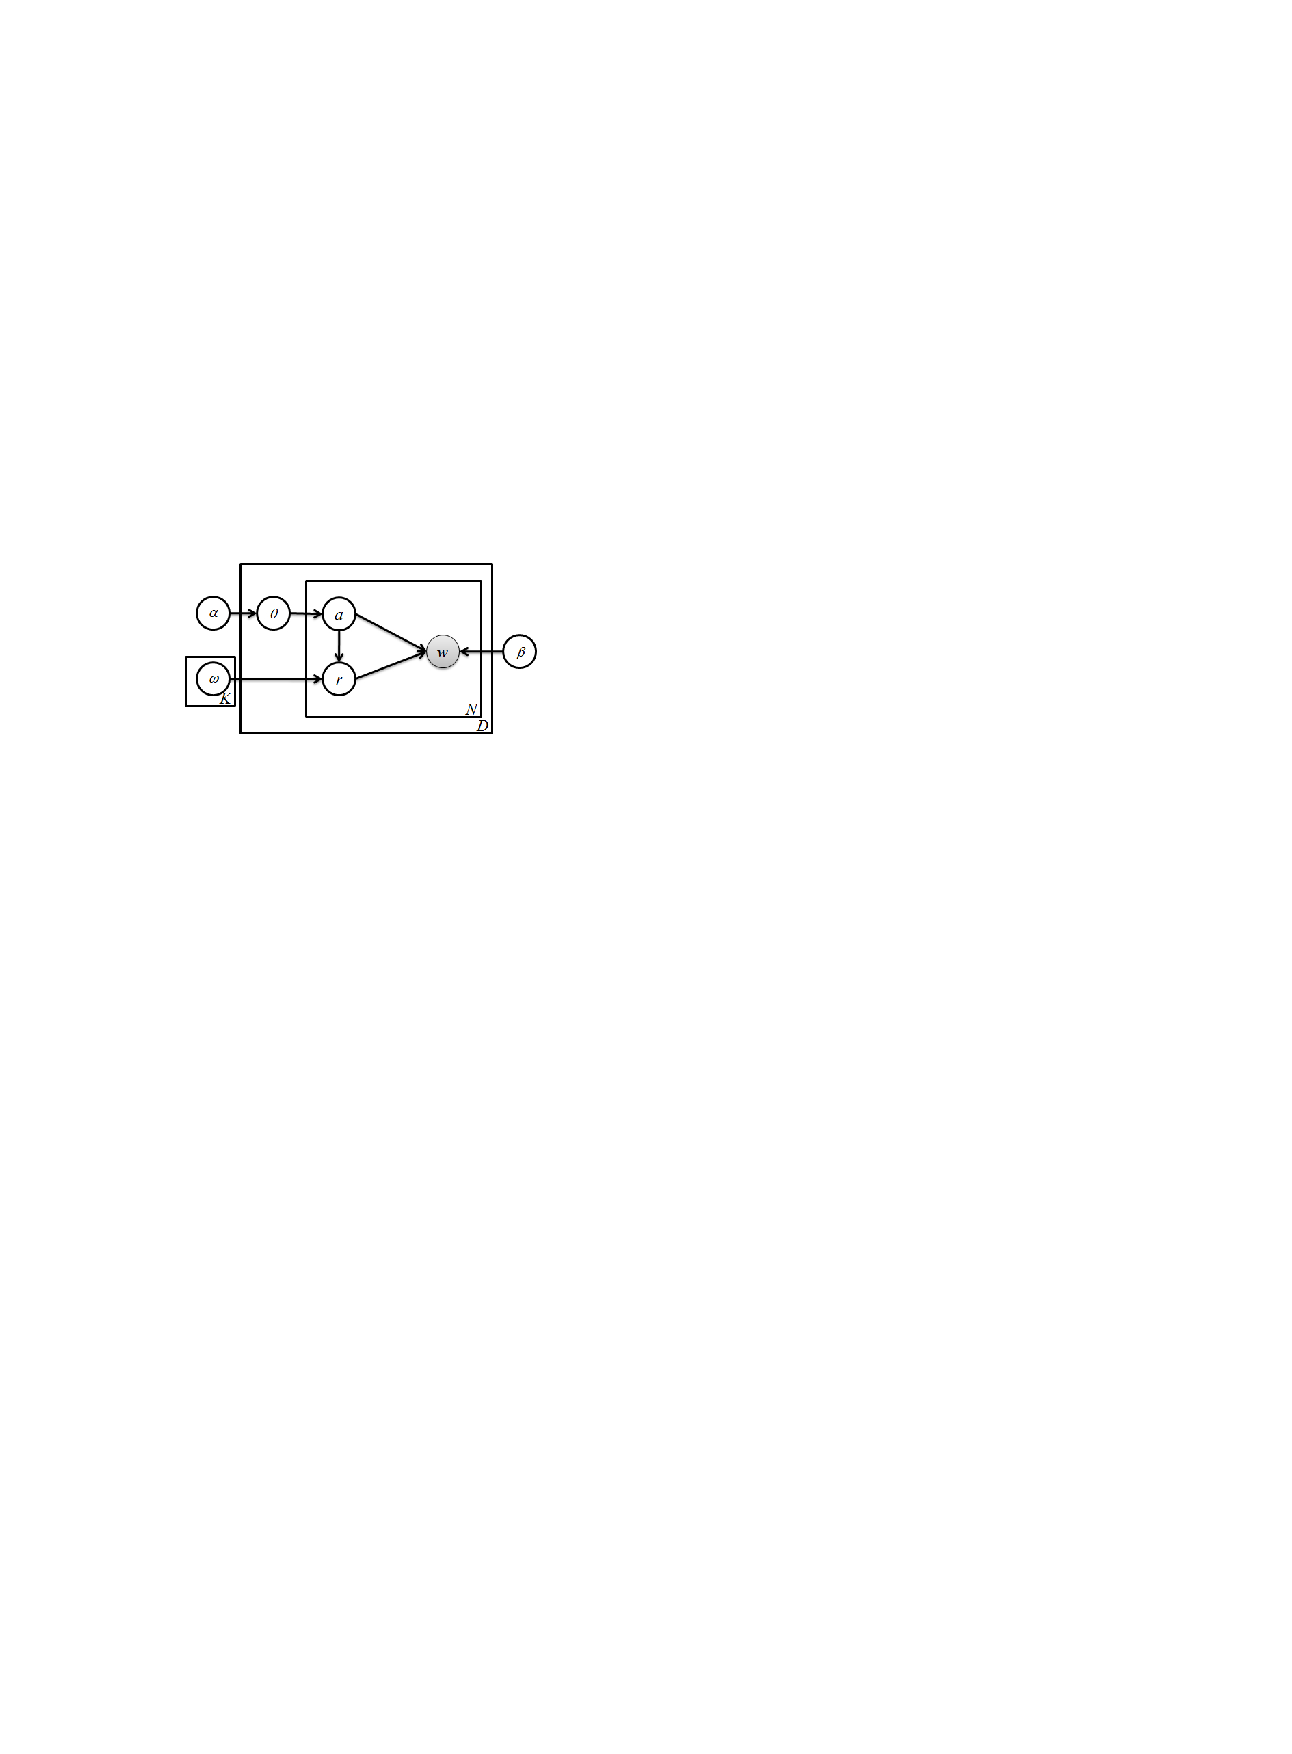
\includegraphics[width=0.5\columnwidth]{figures/methods/D-LDA}
\caption{D-LDA. \cite{moghaddam2012design}}
\label{fig:methods:D-LDA}
\end{figure}

\subsubsection{PLDA: model only opinion phrases}

While LDA assumes that a document is a bag of words, P-LDA \cite{zhan2011semantic,moghaddam2012design} assumes that a document is a bag of opinion phrases. A document is preprocessed to contain only opinion phrases, each being a head-modifier pair $<h_n, m_n>$. Thus, instead of one, the observed variable in P-LDA is two - a head and a modifier, resulting in the generation process as shown in Figure~\ref{fig:methods:P-LDA}:

$$p(\vz, \vh, \vm, \theta | \alpha, \beta, \pi) = p(\theta, \alpha) \prod_{n=1}^N \left[ 
p(z_n| \theta) p(h_n, m_n | z_n, \beta, \pi)\right]$$

\begin{figure}
\centering
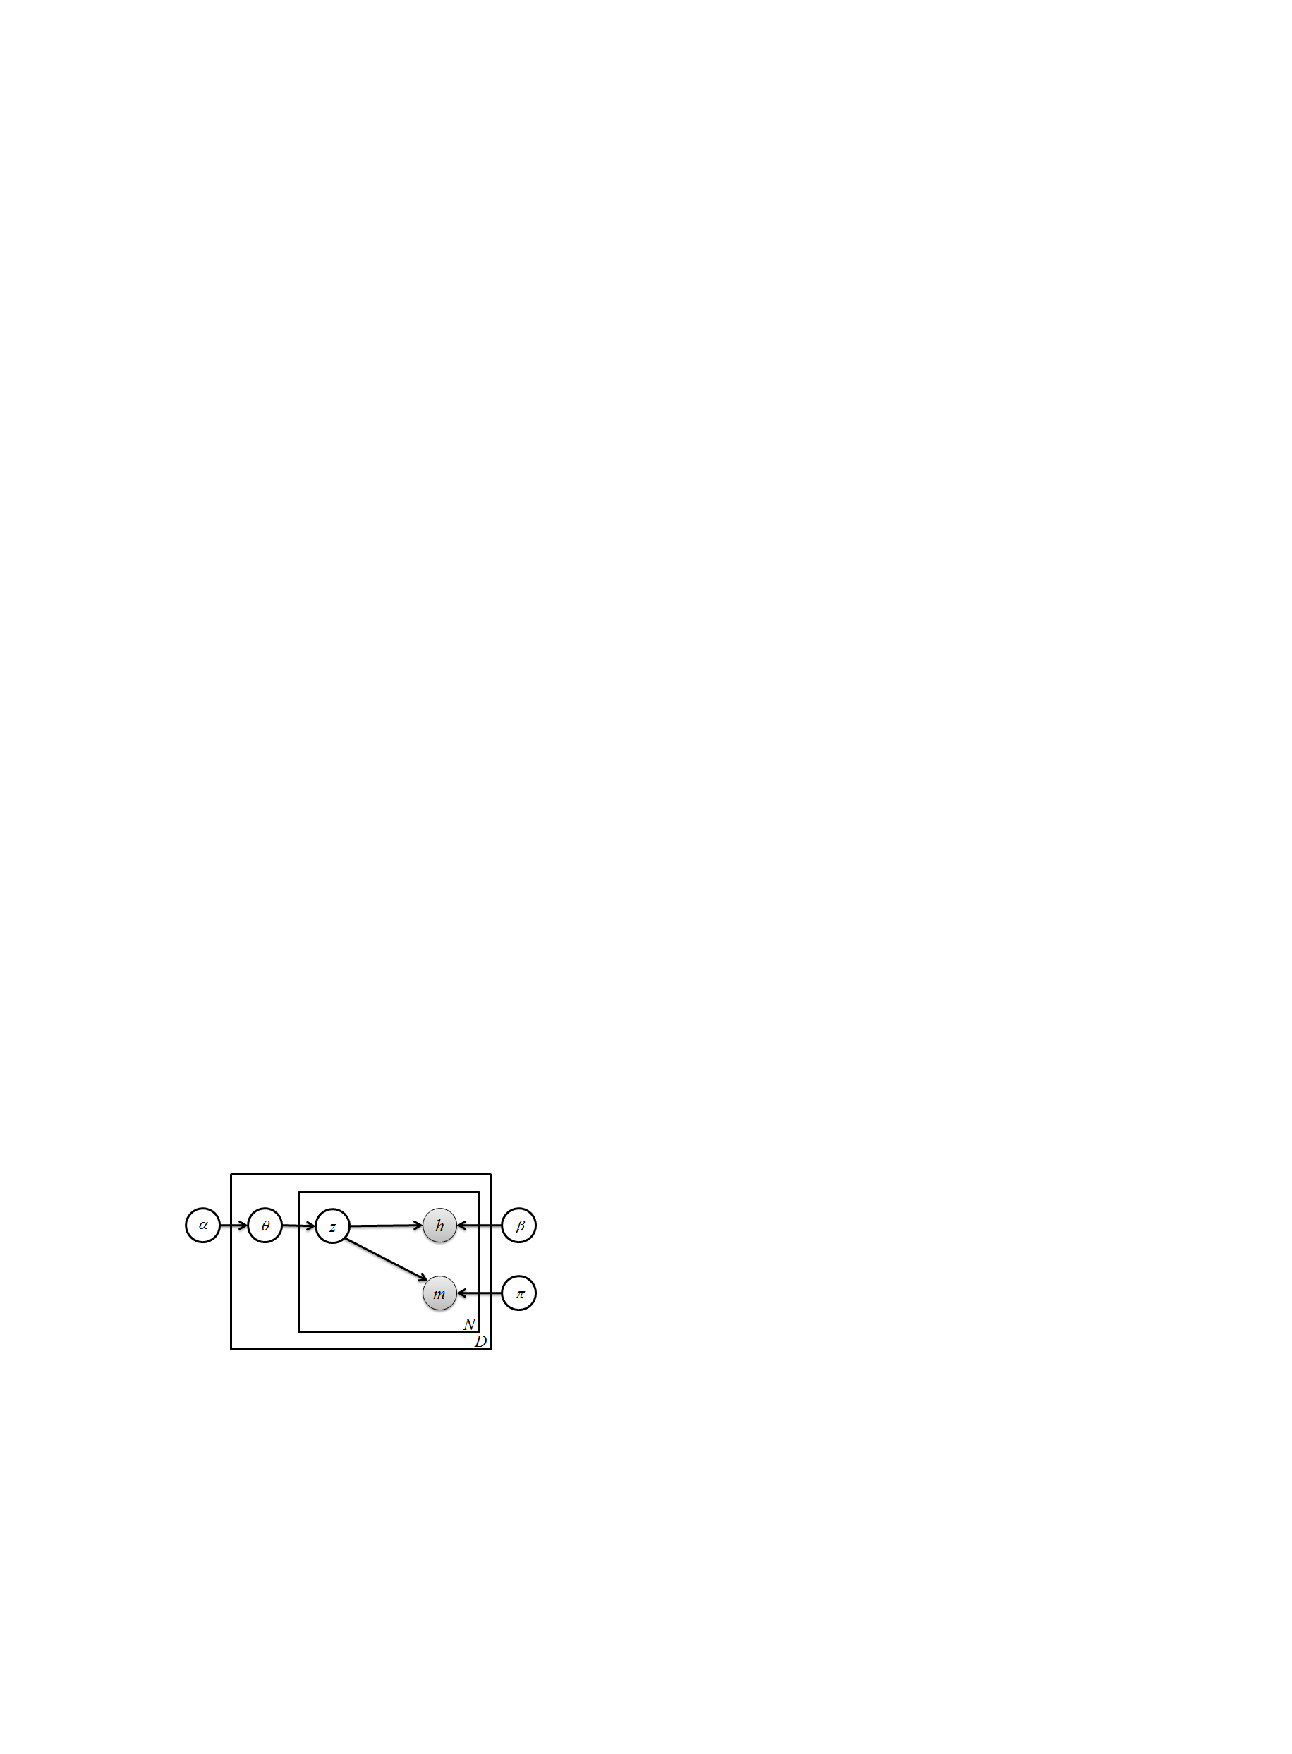
\includegraphics[width=0.5\columnwidth]{figures/methods/P-LDA}
\caption{P-LDA. \cite{moghaddam2012design}}
\label{fig:methods:P-LDA}
\end{figure}

\subsubsection{S-PLDA}

Combining S-LDA and PLDA, we have S-PLDA \cite{moghaddam2012design} as shown in Figure~\ref{fig:methods:S-PLDA}:

$$p(\va, \vr, \vh, \vm, \theta | \alpha, \beta, \pi) = p(\theta, \alpha) \prod_{n=1}^N \left[ 
p(a_n| \theta) p(r_n | \theta) p(h_n | a_n, \beta) p(m_n | r_n, \pi)\right]$$

\begin{figure}
\centering
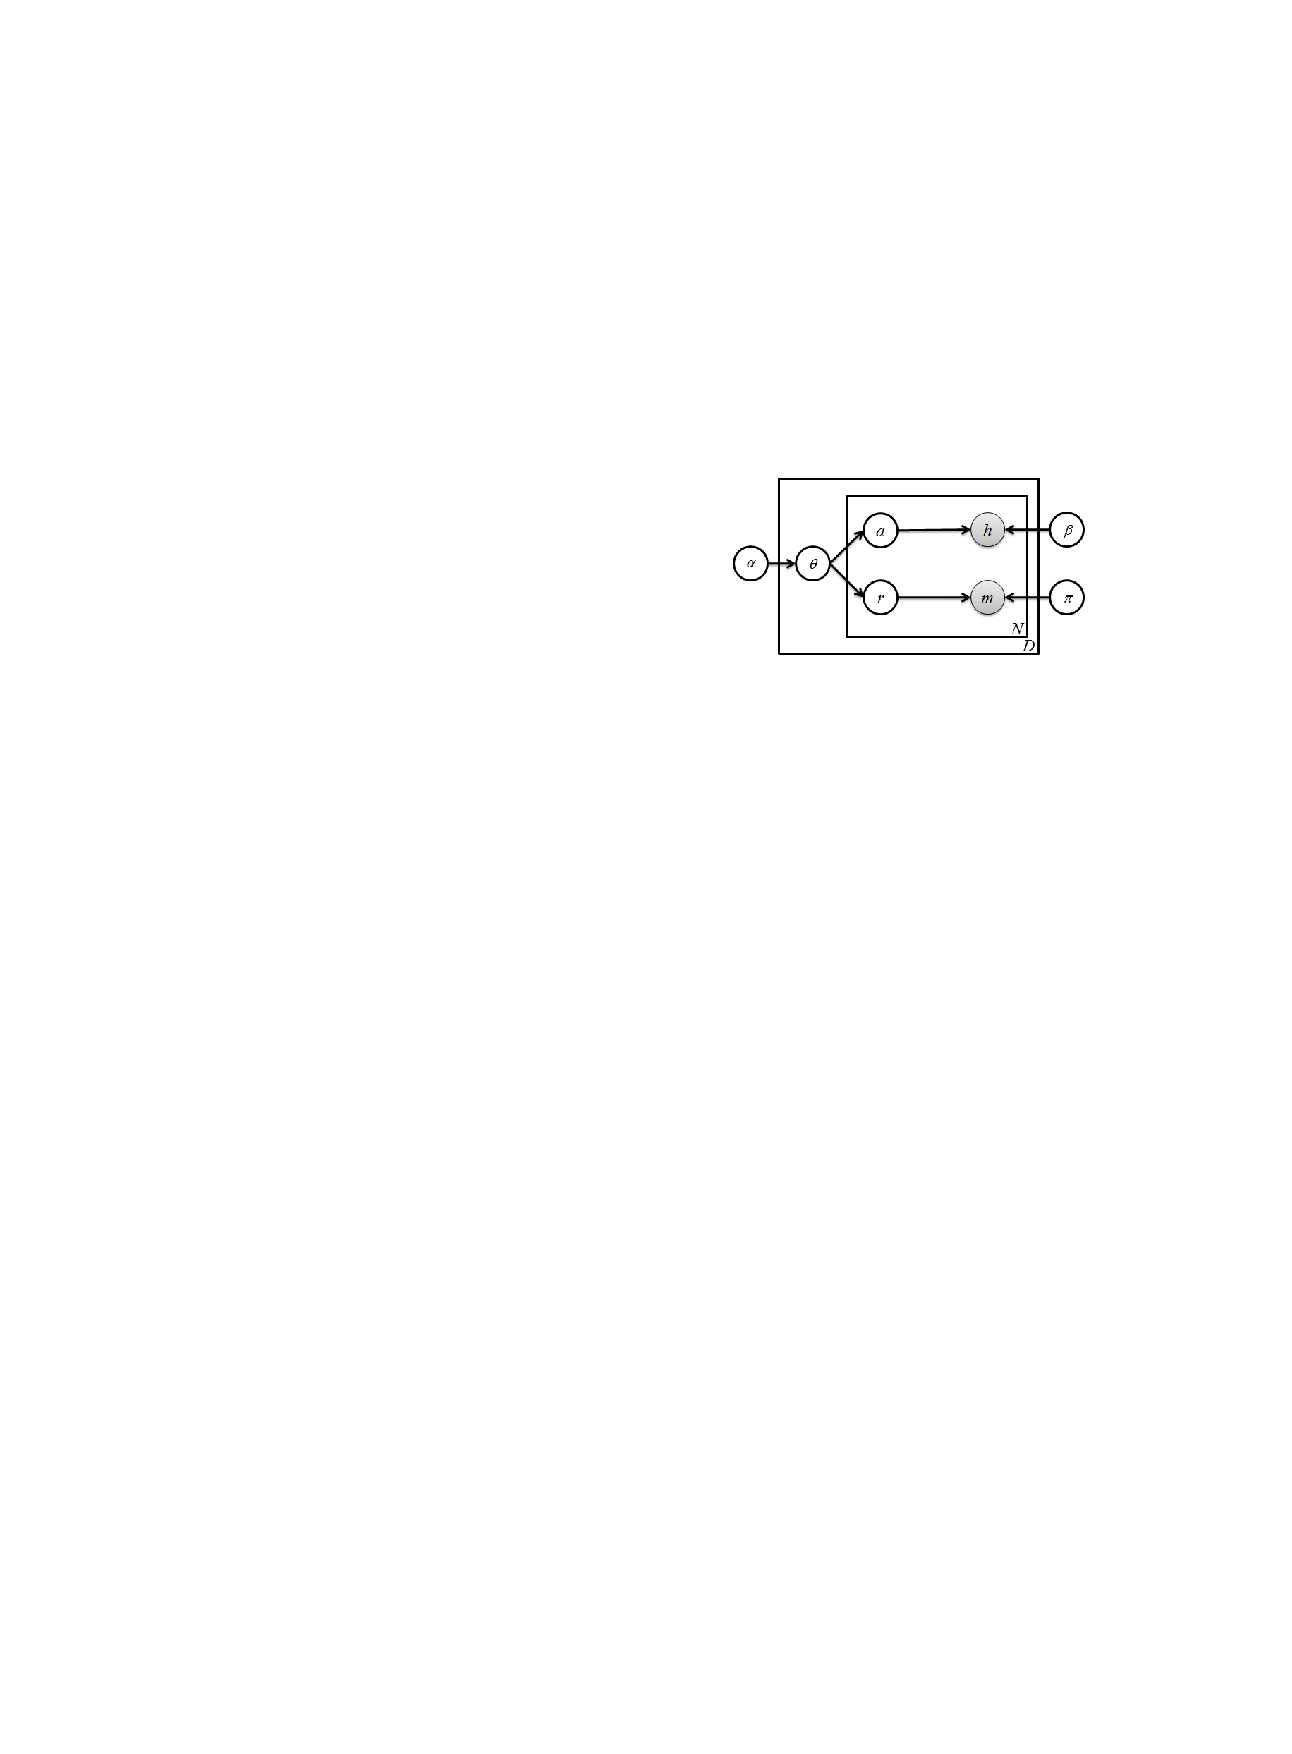
\includegraphics[width=0.5\columnwidth]{figures/methods/S-PLDA}
\caption{S-PLDA. \cite{moghaddam2012design}}
\label{fig:methods:S-PLDA}
\end{figure}

\subsubsection{D-PLDA}

By adding the aspect-rating dependency to S-PLDA, we have D-PLDA \cite{moghaddam2011ILDA,moghaddam2012design}, as shown in Figure~\ref{fig:methods:D-PLDA}:

$$p(\va, \vr, \vh, \vm \theta | \alpha, \beta, \pi) = p(\theta, \alpha) \prod_{n=1}^N \left[ 
p(a_n| \theta) p(r_n | a_n, \theta) p(h_n | a_n, \beta) p(m_n | a_n, r_n, \pi)\right]$$

\begin{figure}
\centering
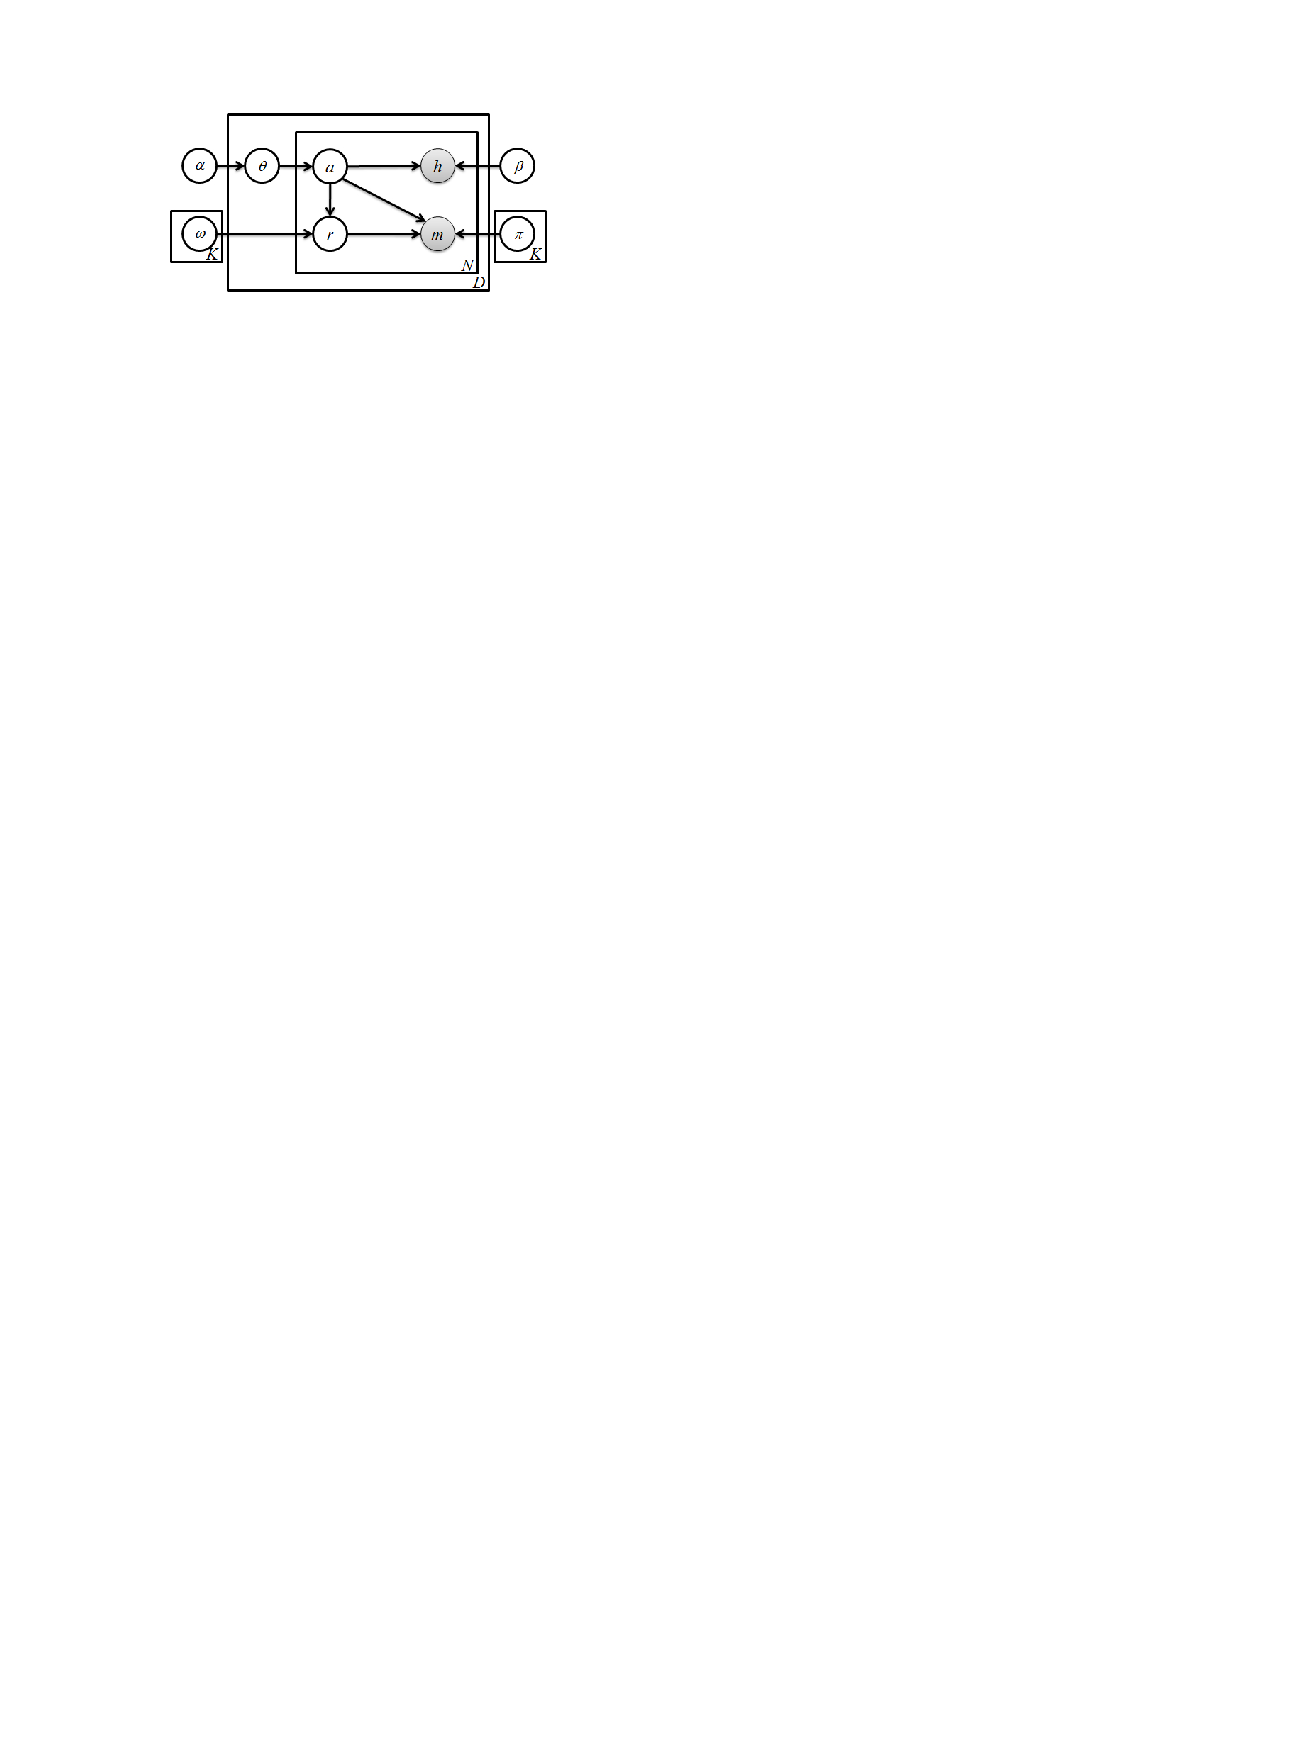
\includegraphics[width=0.5\columnwidth]{figures/methods/D-PLDA}
\caption{D-PLDA. \cite{moghaddam2012design}}
\label{fig:methods:D-PLDA}
\end{figure}

\subsubsection{MG-LDA}

Since aspect extration is a multi-document summarization, the dataset we use is a set of reviews about different products. For example when we perform aspect extraction for hotels, we might use user reviews for different hotel in various cities. Thus in the reviews there are topics that are specific to some particular hotel or a subset of hotels, for example \emph{hotels in Paris}, \emph{youth hostels}. They are valid topics, however not appropriate for ratable aspects. These topics are correlated with the specific product, hence is shared across the scope of the whole review; the topics that can be used as aspects, as analyzed in the previous chapter, are often talked about in segments of the review. The features specific to some product might be prominent at the scope of one review, but if we break down the reivews into sentences, the occurrance of such features specific will be ``diluted" and the aspect topics are more prominent. Motivated by this observation, the authors of MG-LDA \cite{titov2008modeling} introduced two kinds of topics: \emph{local topics} are the ones observed locally in several consecutive sentences, and are appropriate as aspects; \emph{global topics} are the ones closely related to the product and shared across a single review. The generation of words is thus different from that of LDA: now we use a combination of two topic distribution, one global topic that determines the features specific to the product we review, and a local topic that determines which aspect of the product we will talk about. The structure of MG-LDA is shown in Figure~\ref{fig:methods:MG-LDA}. For each document, the global topic distribution is sampled once, since only target product is consistent throughout the review; the local topic distribution is sampled for each sliding window, thus is sampled multiple times across the review, representing the aspect shifting from window to window; each word in a single window is generated by sampling from both topic distributions and combining them.
\begin{figure}
\centering
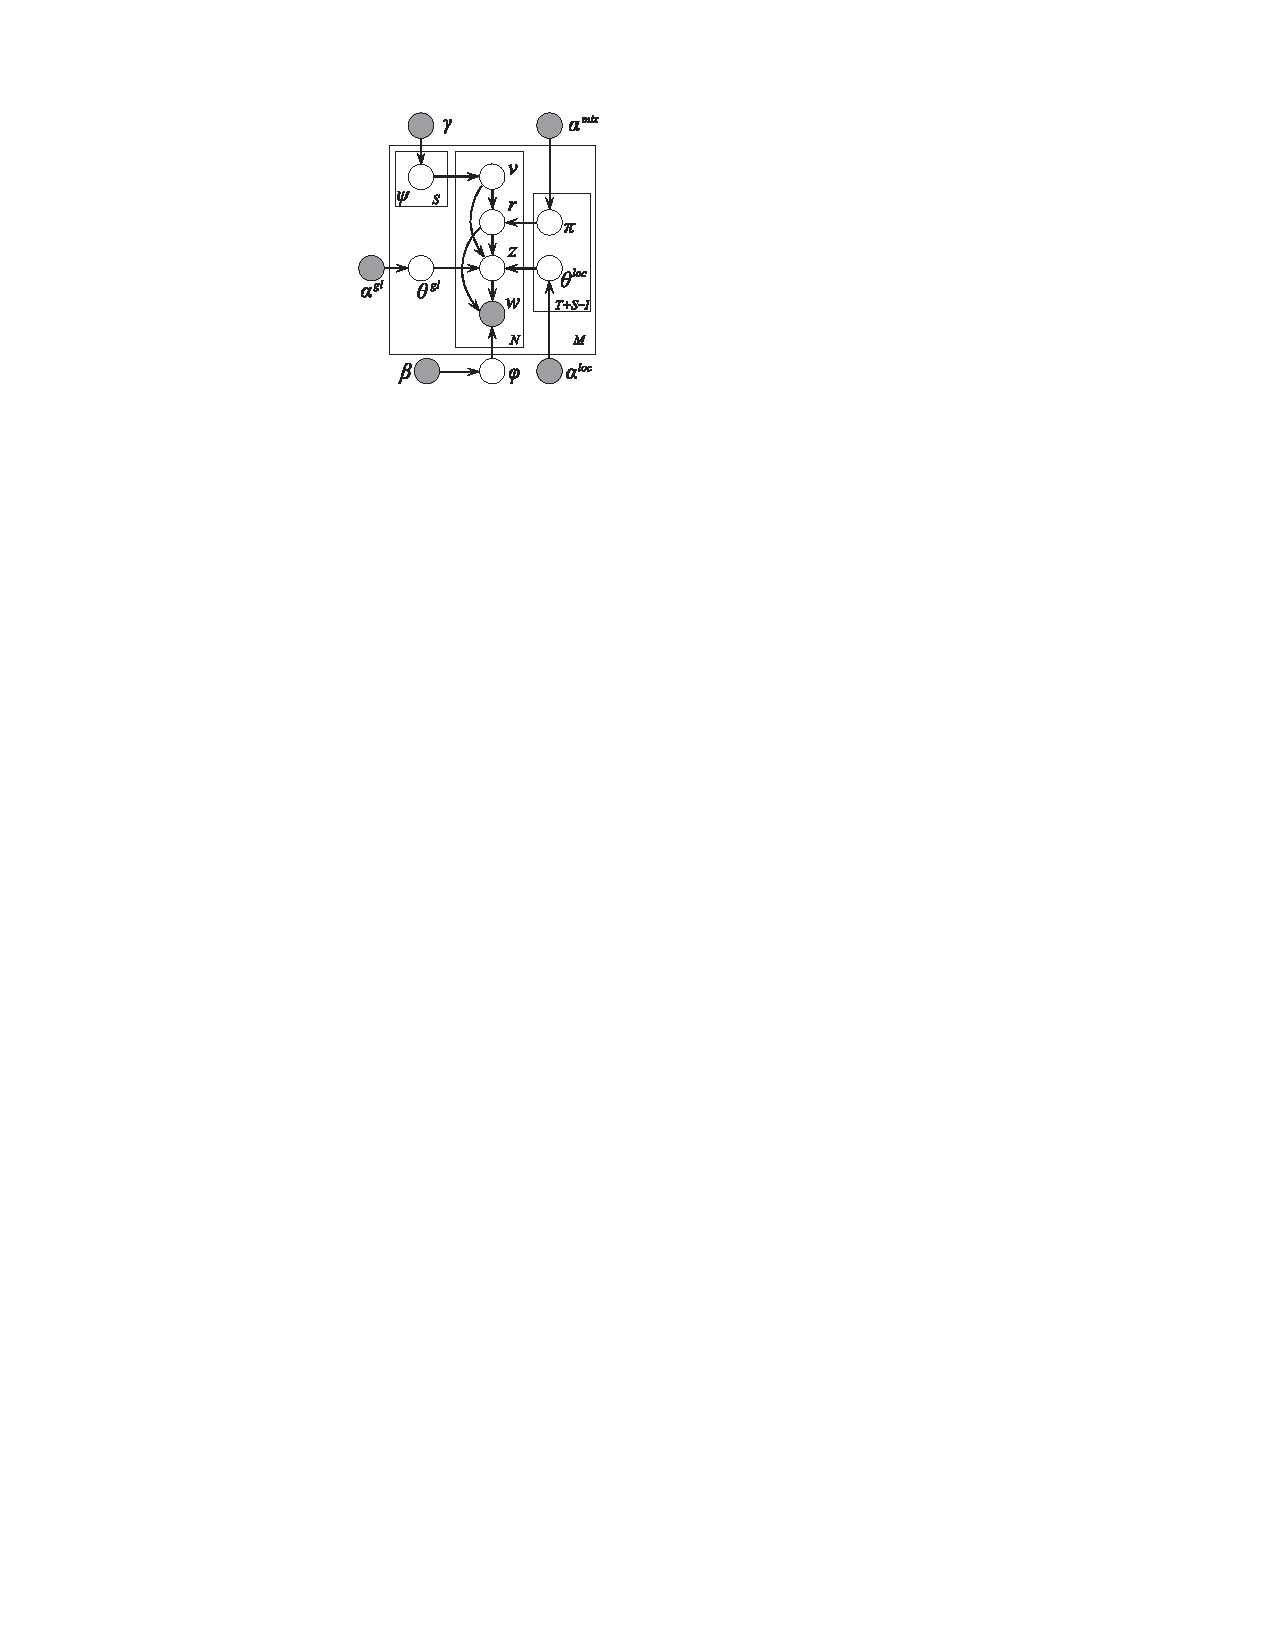
\includegraphics[width=0.5\columnwidth]{figures/methods/MG-LDA}
\caption{MG-LDA. Source of figure: \cite{titov2008modeling}.}
\label{fig:methods:MG-LDA}
\end{figure}

MG-LDA was designed specifically for aspect extraction, without distinguishing aspects and sentiments. MG-LDA has been shown to perform better than other LDA variations mentioned above, so we will make a direct comparison with our model  in our experiment chapter.

\section{Deep Learning for Natural Language Processing}


\begin{displayquote}
 ``Deep Learning waves have lapped at the shores of computational linguistics for several years now, but 2015 seems like the year when the full force of the tsunami hit the major Natural Language Processing (NLP) conferences." - Dr. Christopher D. Manning, Dec 2015 
\end{displayquote}

Deep learning has drawn a lot of attentiono in recent years, and we have already seen many applications of it in natural language processing. In this section we will first give a brief introduction to the history of deep learning; then we will introduce several widely used deep learning methods for natural language processing. 

\subsection{A Brief History of Deep Learning}

The core model of deep learning is neural network. The earliest neural-network-like algorithms that had multiple layers of no-linear features can be traced back to \cite{ivakhnenko1965cybernetic}, where the authors used a thin but deep models with polynomial activation functions which they analyzed with statistical methods. In each layer, they select the best features through statistical methods and forward them to the next layer. They did not use backpropagation to train their network end-to-end but used layer-by-layer least squares fitting where previous layers were independently fitted from later layers.

The earlist convolutional network appeared in \cite{fukushima1979organization}. Their networks had multiple convolutional and pooling layers similar to modern networks, but the network was trained by using a reinforcement scheme where a tail of strong activationo oin multiple layers was increased over time.

Backpropagation of erros that are used to train deep models was lacking at this point. It was derived already in the early 1960s but in an inefficient and incomplete form. The modern form was derived first by Linnainmaa in his 1970 masters thesis, however he did not mention its application to neural networks. Even at this point, backpropagation was relatively unknown and very few documented applications of backpropagation in the early 1980s. \cite{rumelhart1988learning} showed that backpropagation used for neural networks could yield interesting distributed representations. At this time, this was an important result in cognitive psychology where the questiono was whether human cognition can be thought of as relying on distributed representations (connectionism) or symbolic logic (computationalism).

The first practical application of backpropagation cam about through \cite{lecun1989backpropagation} where the authors used convolutional networksin combination with backpropagation to classify handwritten digits (MNIST) and this system was later used to read large numbers of handwritten checks in the United States. Despite these successes, funding for research into neural networks was scarce. The term artificial intelligence dropped to near pseudoscience status during the ``AI winter". Some important advances were made in this time, for example, long short-term memory (LSTM) for recurrent neural network \cite{hochreiter1997long}, but these advances went mostly unnoticed util later as they were overshadowed by support vector machine (SVM) \cite{cortes1995support}.

The next big shift occured just by waiting for the computers to get fater, and then later by the introduction of GPU. In this period, neural networks slowly began to rival SVMs. The main difficulty at this point was to train big, deep networks, which suffered from vanishing gradient problem, where features in early layers could not be learned because no learning signal reached these layers.

The first solution to this problem was layer-by-layer pre-training, where the model is built in a layer-by-layer fashion by using unsupervised learning method. The first pre-training approaches was proposed for recurrent neural networks by \cite{schmidhuber1992learning}, and then for feed-forward networks by \cite{hinton2006reducing}, which started the fever of neural networks.

\subsection{Word2Vec}

As natural language processing often treats words as the basic unit of study and neural networks takes vectors as input, it is natural to represent words by vectors. The most basic model is one-hot vector, where each vector has the size of the vocabulary, and one non-zero entry denoting the word. This simple design has several drawbacks: first it's dimensionality is too large if we have a large dictionary; secondly and more importantly, the vector representation does not capture any semantic information of the words. To improve the vector representation of words, we replace the original high-dimensional discrete vector with a lower-dimensional real-valued vector; instead of the pre-defined fixed values, we train the vector representations so that the cosine similarity of two word vectors captures the semantic similarity of the two corresponding words. This Word2Vec \cite{mikolov2013distributed} model adopted a heuristic: if two words often appear close to each other, then they are similar, and this is called word embedding - embed a word's meaning in the the words surrounding it. Also, the semantics of each word is stored in all the entries of the word vector, so the word vector we learned is called a \emph{distributed representation}.

Word2Vec contains two seperate models: skip-gram and CBOW. The two models can used independently two train two vectors for each word, and concatenate the two vectors to obtain the final word embedding. However in practice, people often use only the skip-gram model with special training techniques like negative samping and noise contrastive estimation. In our paper, we introduce skip-gram with negative sampling.

For a high level interpretation, we consider a single word $w$ in a sentence: skip-gram asks us to predict each other word, or context word $c$, in the sentence with $w$; this way we embed the meaning of the context in the representation of $w$. For a more formal definition, we consider all the word-context pairs $(w,c)$ in a corpus $D$, and we consider the conditional probabilities $p(c|w)$. We use $C(w)$ to denote the set of contexts of word $w$, and $\theta$ as the parameters of $p(c|w; \theta)$. Our goal is to find the parameters that maximize the corpus probability.

$$\theta = \argmax_{\theta} \prod_{w\in W} \left[\prod_{c\in C(w)} p(c|w; \theta) \right]\text{;  or alternatively}$$
$$\theta = \argmax_{\theta} \prod_{(w,c)\in D} p(c|w; \theta)$$

When predicting each context word $c$ with word $w$, the model uses a softmax:

$$p(c|w;\theta) = \frac{e^{v_c\cdot v_w}}{\sum_{c'\in C}e^{v_{c'}\cdot v_w}}$$

where $v_c, v_w, v_{c'} \in \mathbb{R}^d$ are vector representations of $c, w, c'$ respectively; $C$ is the set of all available contexts. Maximizing the above conditional probability is equivalent to maximizing the objective:

$$\argmax_{\theta}\sum_{(w,c)\in D} \log p(c|w)
= \sum_{(w,c)\in D} (\log e^{v_c\cdot v_w} - \log\sum_{c'\in C}e^{v_{c'}\cdot v_w})$$

While the above objective can be computed, but it's computationally expensive to do so, because the summation will iterate over all the contexts $c'$. One way of making the computation more tractable is to replace the summation with a sampling of random noises, this is called negative sampling. Note that other methods like noise contrastive estimation \cite{mnih2013learning} and importance sampling \cite{bengio2003quick,bengio2008adaptive} all share the same basic idea, and we will not elaborate on thess two other models in this paper.

With negative sampling, the model is actually optimizing a different objective. Consider a word-context pair $(w,c)$, we denote by $p(D=1|w,c)$ the probability that $(w,c)$ came from the corpus, correspondingly, $p(D=0|w,c)=1-p(D=1|w,c)$ denotes the probability did not come from the corpus. Still with parameters $\theta$, our goal is now to maximize the probabilities that all the observed pairs indeed came from the corpus:

\begin{align*}
    &\argmax_{\theta}\prod_{(w,c)\in D} p(D=1|w,c;\theta) \\
    &=\argmax_{\theta} log \prod_{(w,c)\in D} p(D=1|w,c;\theta) \\
    &=\argmax_{\theta} \sum_{(w,c)\in D} \log p(D=1|w,c;\theta)
\end{align*}

The conditional probability $p(D|w,c|\theta)$ is defined using softmax:

$$p(D=1|w,c;\theta)=\frac{1}{1+e^{-v_c\cdot v_w}}$$

leading to the objective:

$$\argmax_{\theta}\sum_{(w,c)\in D}\log \frac{1}{1+e^{-v_c\cdot v_w}}$$

This objective has a trivial solution if we set $\theta$ so that $v_c=v_w$ and $p(D=1|w,c;\theta)=1$ all the time. But we of course don't want all the words share a same representation and we will disallow some $(w,c)$ pairs. One way to do so is to make $p(D=1|w,c;\theta)$ low for some pairs, i.e. pairs not observed in the data. This is achieved by generating the set $D'$ of random $(w,c)$ pairs and assuming they are out of the corpus - hence ``negative samples". Let $\sigma(x)=\frac{1}{1+e^{-x}}$, the new objective is:

\begin{align*}
    &\argmax_{\theta}\prod_{(w,c)\in D} p(D=1|w,c;\theta) \prod_{(w,c)\in D'}p(D=0|w,c;\theta) \\
    =&\argmax_{\theta}\prod_{(w,c)\in D} p(D=1|w,c;\theta) \prod_{(w,c)\in D'}(1-p(D=1|w,c;\theta)) \\
    =&\argmax_{\theta}\sum_{(w,c)\in D} \log p(D=1|w,c;\theta) + \sum_{(w,c)\in D'} \log(1-p(D=1|w,c;\theta)) \\
    =&\argmax_{\theta}\sum_{(w,c)\in D} \log\sigma(v_c\cdot v_w) + \sum_{(w,c)\in D'} \log\sigma(-v_c\cdot v_w)
\end{align*}

This model can then be trained end-to-end much more efficiently and the final parameters $\theta$ contains all the word vectors. This objective has been shown to be equivalent to factorizting a shifted PMI matrix \cite{levy2014neural}, which means that the semantic similarity captured by Word2Vec is actually the point-wise mutual information between the pair of words. Their are other models of vector representation for words, including \cite{pennington2014glove,shazeer2016swivel}, but Word2Vec is by far the most widely used word vector in applications.


\subsection{Neural Network Language Model}

The goal of statistical language model is to learn the joint probability function of sequences of words in a language. This is difficult due to the curse of dimensionality: there are too many possible sequences. Traditional approaches based on n-grams obtain generalization ability by concatenating very short overlapping sequences, focusing on only a local window each time. In neural network language models, the index-based word representation used in traditional n-gram models is replaced with distributed representations like Word2Vec. This allows the model to be informed about an exponential number of semantically neighboring words each time, due to the semantic embedding in each word vector. With word vectors, the model simultaneously learns the representation of each word and the probability function of the sequence. The generalization ability is improved because each word now shares its information with many other similar words, replacing a word in a already seen sequence with a semantically similar word will now result in a similar probability function.

A statistical language model can be defined by the conditional probability of the next word given previous words: $p(w_1^T) = \prod_{t=1}^T p(w_t | w_1^{t-1})$. The earliest neural network language model was proposed in \cite{bengio2000a} and follows the n-gram approach, which means that it approximate the conditional probability:

$$p(w_t | w_1^{t-1}) \approx p(w_t | w_{t-n+1}^{t-1})$$

The modeling of function $f(w_t,..., w_{t-n+1}) = p(w_t | w_1^{t-1})$ is done by two steps:

\begin{itemize}
    \item[1.] By using a matrix $C$ of shape $|V|\times m$, where $V$ is the vocabulary and $m$ is the dimension of word vector, we map the input sequence $(w_{t-n+1}, ..., w_{t-1})$ to a sequence of word vectors $(C(w_{t-n+1}), ..., C(w_{t-1}))$;
    \item[2.] A function $g$ maps the input sequence of word vectors to a conditional probability distribution over all the words in $V$ for the next word $w_t$. The output is a probability vector whose $i$th element estimates $p(w_t=i|w_1^{t-1})$.
\end{itemize}
$$f(i, w_{t-1}, ..., w_{t-n+1}) = g(i, C(w_{t-1}), ..., C(w_{t-n+1}))$$

Note that among the two mappings $g$ and $C$, the later is shared across all the words in the context, holding all the $|V|$ word vectors in rows. Function $g$ is designed to be a feed-forward neural network with parameters $\omega$, so the whole parameter set is $\theta={C, \omega}$. The objective is to minimize the log-likelihood of the entire corpus ($T$ word sequences):

$$L=\frac{1}{T} \sum_t \log f(w_t, w_{t-1}, ..., w_{t-n+1}; \theta) + R(\theta)$$

where $R(\theta)$ is a regularization term designed for avoiding over-fitting of the neural network. 

The input layer of the network receives the sequence of words, map them into a sequence of word vectors and pass it to a normal tangent hidden layer and obtain the outputs $y_i$ for word $i$. The output layer, similar to what is used in skip-gram in Word2Vec, is a softmax output layer:

$$p(w_t | w_{t-1}, ..., w_{t-n+1}) = \frac{e^{y_{w_t}}}{\sum_i e^{y_i}}$$

where $y$ is given by the hidden layer computation:

$$y=b+Wx+U\tanh(d+Hx)$$

where the hyperbolic tangent is applied element-wise; $x$ is the concatenation of the input word vectors:

$$x=(C(w_{t-1}), C(w_{t-2}), ..., C(w_{t-n+1}))$$

The whole model is then trained end-to-end, simultaneously learning the representation of words and the probability function for sequences.

The model has several restrictions to this language model that is based on a feed-forward neural network. First the computational cost at the softmax layer is very high, similar to what we see from Word2Vec, but this time we cannot directly use negative sampling, because we need to consider the $n-1$ previous words, instead of only one word. Importance sampling can be applied to this scenario with some careful modification \cite{cho2015on}. Another way to solve this problem is to replace the flat softmax with some hierarchical structure, that is, using a hierarchical softmax \cite{mikolov2013efficient}. Also the normalization of the softmax can be replaced by a self-normalizing term learned jointly with the model \cite{devlin2014fast}. Beside the computational efficiency, this model is restricted to using local features - only previous $n-1$ words are used for predicting the next word. To address this problem, we adopt recurrent neural network, which is specifically designed for modeling sequences of different lengths.

\subsection{Recurrent Neural Network}

The idea behind recurrent neural network (RNN) is to make use of sequential information. In traditional layer structured neural network, we assume that all inputs (and outputs) are independent of each other. But for tasks like language modeling this is a huge restriction. RNN is ``recurrent" because it performs the same process for every element in a sequence, with the output being depended on the previous computations. Another way to think about RNN is that it has a ``memory" which captures imformation about what has been calculated so far. In theory RNN can make use of information in arbitrarily long seuqnces, but inpractive they are limited to looking back only a few steps.

The computation of RNN is slightly different from normal neural network which is a stack of layers, instead of going through the fixed structure of layers, RNN carry out its computation in multiple time steps. The time steps of RNN actually correspond to the layers of normal neural network, however the depth of layers is not pre-defined and varys according to the input sequence. RNN has two core functions which it performs at each time step: update of its internal state, and output based on its internal state; the later is optional.

The abstraction of RNN internal state update is simple: $h_t=\RNN(h_{t-1}, x_t)$, where $h_t$ is the new state, $h_{t-1}$ is the previous state, $x_i$ is the input at this time step, all of them are vectors; $\RNN$ encapsules the computation of an RNN layer, which in the most simple form is just linear transformations followed by a non-linearity (biases are dropped for simplicity):

$$RNN(h_{t-1}, x_t) = tanh(Wh_{t-1} + Ux_t)$$

The output part of RNN is also simple. Let us consider the scenario of language modeling. At each time step $t$ we have a hidden state $h_t$ which contains the information of all previous words $(x_1, ..., x_t)$. With this state we can predict the next word $x_{t+1}$ by computing a softmax over all possible words, which gives us the probability of next word $x_{t+1}$ conditioned on the previous words, therefore we can model the probability of the whole sequence with this RNN. After training the RNN for language modeling, it can be further used for generating sequences: at each time, take the word with the highest probability predicted by the softmax; then feed the predicted output to the RNN as an input; proceed until the RNN outputs a special symbol denoting the end of the sequence.

\begin{figure}
\centering
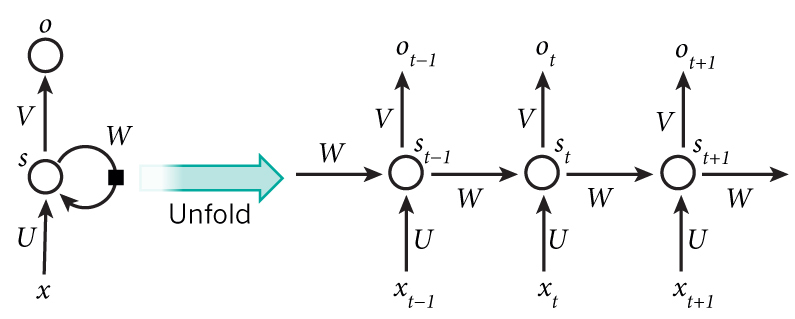
\includegraphics[width=0.7\columnwidth]{figures/methods/RNN}
\caption{The rolled and unrolled forms of RNN. Source: \emph{Nature}.}
\label{fig:methods:RNN}
\end{figure}

The rolled and unrolled forms of RNN is shown in Figure~\ref{fig:methods:RNN}. It is important to remember that almost all RNN structures follow the abstraction above, though the instantiation of the $\RNN$ function might be much more complicated. With this abstraction, we can see the correspondence between RNN and a traditional neural network structure: the hidden states of RNN correspond to the activations of a normal NN's hidden layers, but the parameters are shared across layers. This correspondence leads us to the training algorithm for RNN - backpropagation through time (BPTT). After unrolling the RNN computation into layers similar to normal NN, we do backpropagation just like normal; but after updating the weights at all the layers - which are actually copies of a single layer, we take the average of those copies and use it as the new RNN layer.

Since RNN and normal NN use virtually the same training algorithm, the difficulty of training a deep neural network also occurs to RNN when the input sequence is long and the depth of RNN is correspondingly large. The main problem is the vanishing gradient problem \cite{hochreiter1991untersuchungen,hochreiter2001gradient}. The intuitive explaination of vanishing gradient is: RNN updates involves repeatedly multiplying a matrix to itself, and when the matrix entries are small, almost no gradient is passed to earlier layers. The result is: information learned at later time steps cannot be efficiently passed to earlier time steps, making it hard for RNN to learn long-distance dependencies in the sequence. Detailed analysis of the vanishing gradient problem can be found in \cite{pascanu2013on}. This problem makes RNN less useful for something like language modeling, which often involves long input sequences.

\subsubsection{Long Short-Term Memory}

Long Short-Term Memory \cite{hochreiter1997long} is a variation of RNN that is designed to address the vanishing gradient problem. The abstraction of LSTM is still the same to the original one: $h_i=\RNN(h_{t-1}, x_t)$; however the update function $\RNN$ is more complicated. LSTM introduced four new elements: input gate $i$, forget gate $f$, output gate $o$, and cell $c$; the formal update function is:

\begin{align*}
& i_t = \sigma(W^i x_t + U^i h_{t-1}) \\
& f_t = \sigma(W^f x_t + U^f h_{t-1}) \\
& o_t = \sigma(W^o x_t + U^o h_{t-1}) \\
& c_t = f_t \odot c_{t-1} + i_t \odot \tanh(Wx_t + Uh_{t-1}) \\
& h_t = o_t \odot \tanh(c_t)
\end{align*}

where $\sigma$ is the sigmoid function, $\odot$ denotes the element-wise product.

Despite the seemingly complicated design, there is a clear intuition behind LSTM. LSTM can be derived from normal RNN by two steps:

\begin{itemize}
    \item[1.] In the original RNN, the repeated multiplication introduced the vanishing gradient problem, so we replace the multiplications with additions. This is done by introducing the cell and update it with addition.
    \item[2.] There are three projections in RNN and we take care of them by using the three gates, so the model has the flexibility of deciding what informationo to pass to the next time step:
        \begin{itemize}
            \item input to hidden: input gate
            \item hidden to hidden: forget gate
            \item hidden to output: output gate
        \end{itemize}
    Now the cell keeps the real memory (hence the real ``hidden state"), and the hidden state is what the cell exposes to the next time step.
\end{itemize}

\begin{figure}
\centering
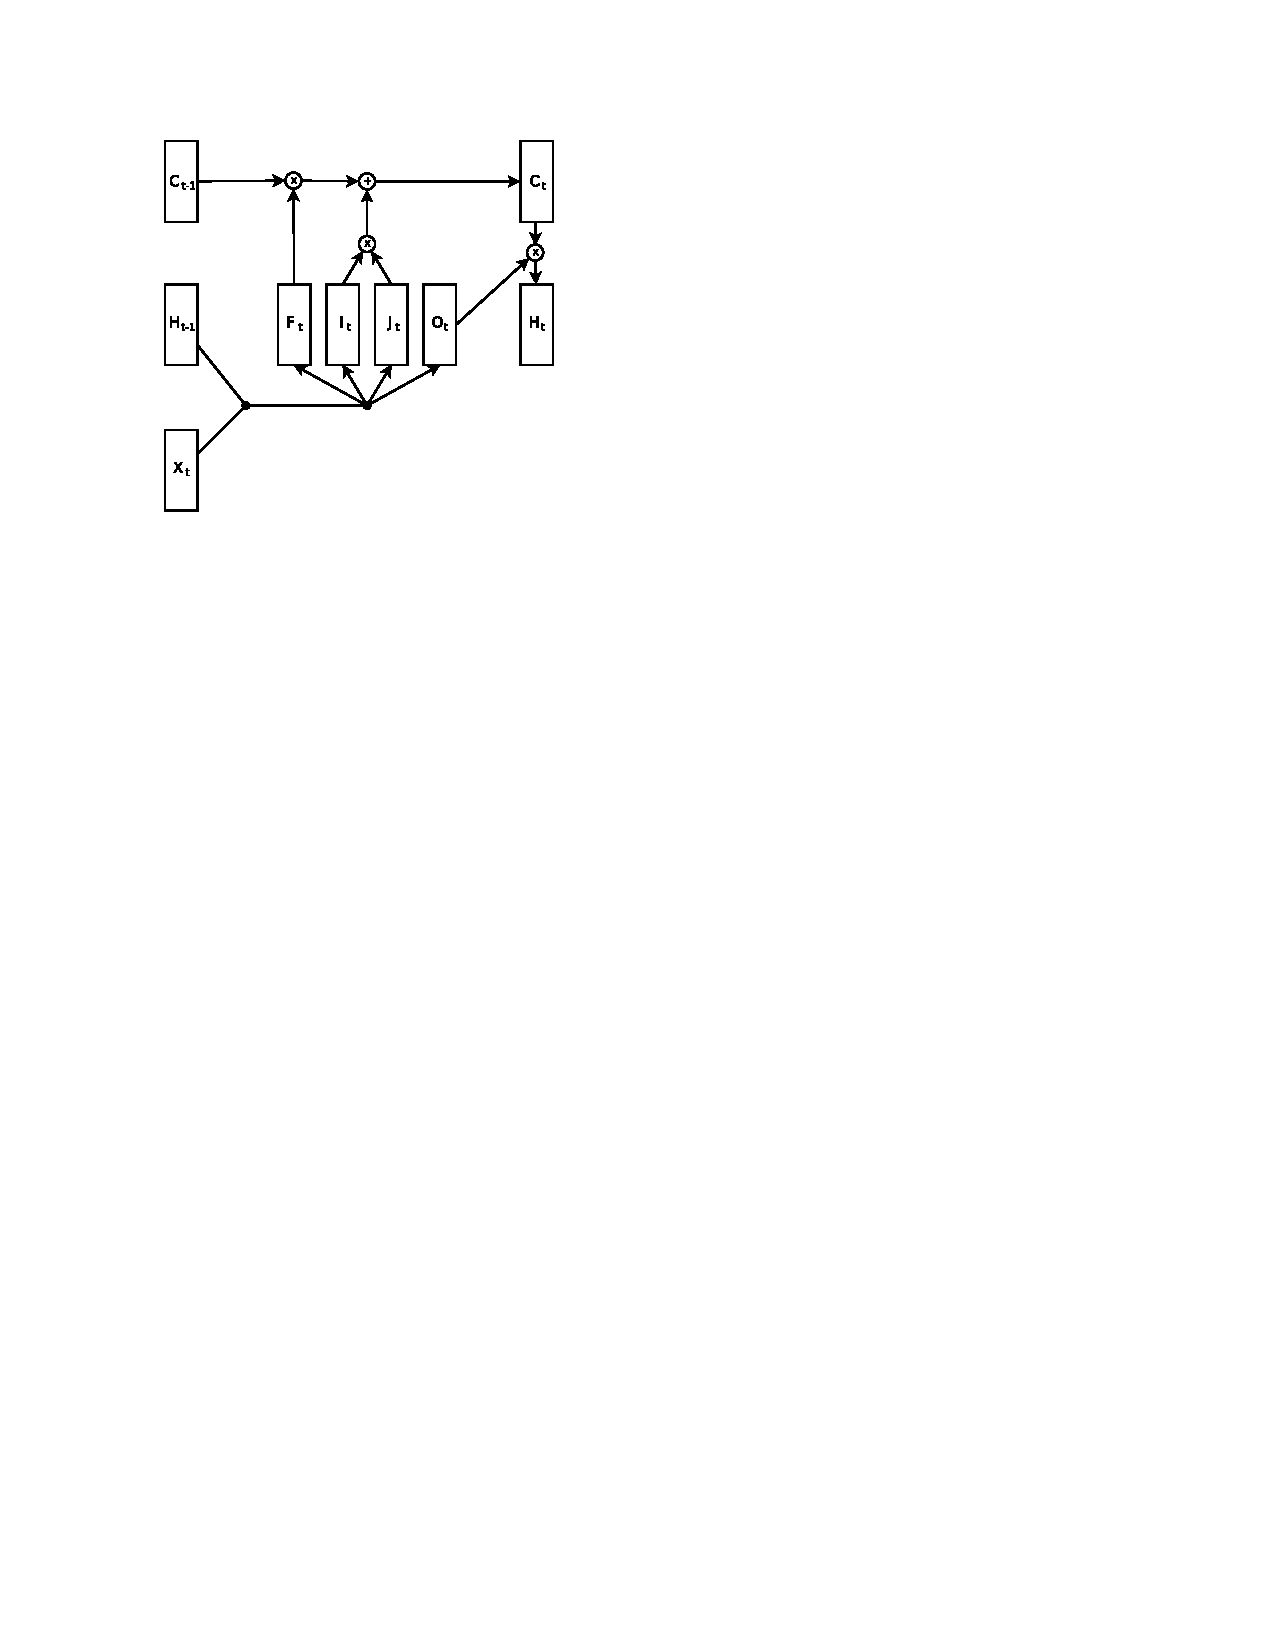
\includegraphics[width=0.7\columnwidth]{figures/methods/LSTM}
\caption{Long Short-term Memory. Source of figure: \cite{jozefowicz2015empirical}.}
\label{fig:methods:LSTM}
\end{figure}

The structure of LSTM is shown in Figure~\ref{fig:methods:LSTM}. The use of the gates is to allow the corresponding projection keep the original signal without applying any non-linearity, enabling part of the model to perform an identity mapping. Similar idea is recently applied to normal neural network by introducing ``residual connection", which is basically an identity mapping in addition to the original non-linear transformation. This significantly improved the performance of very deep neural netowrks (as deep as a thousand layers), related works can be found in \cite{srivastava2015highway, he2015deep, huang2016deep}.


\subsection{Paragraph Vector}
\label{section:paragraph_vector}
Using recurrent neural network is only one of the methods of sequence modeling. There are other methods which try to extend word2vec to phrase and sentence level. Given a vector representation of words, the most direct way of representing a sentence is taking the average of the corresponding word vectors. But this is obviously too simple, for the following reasons:

\begin{itemize}
    \item The words in a sentence should not be treated with equal attention. Different words are of different significance to the semantics of the sentence, hence in making the sentence representation, we should not use the same weight for all the words.
    \item The word order information is lost in this simple representation. Note that with the same set of words, different orders can render completely different meanings.
\end{itemize}

One way of making a better sentence representation is to leverage the parsing tree. In\cite{socher2011parsing}, the authors used a recursive neural network to process the parsing tree and build up the sentence representation along the tree structure. However this approach only works for sentences with good grammar because the final vector representation relies highly on the quality of the parsing tree.

In \cite{le2014distributed}, the authors proposed a much less complicated method which is a simple extension to the two models from word2vec, called paragraph vector. We will introduce the two extended models in the following.

\subsubsection{PV-DM}

\begin{figure}
\centering
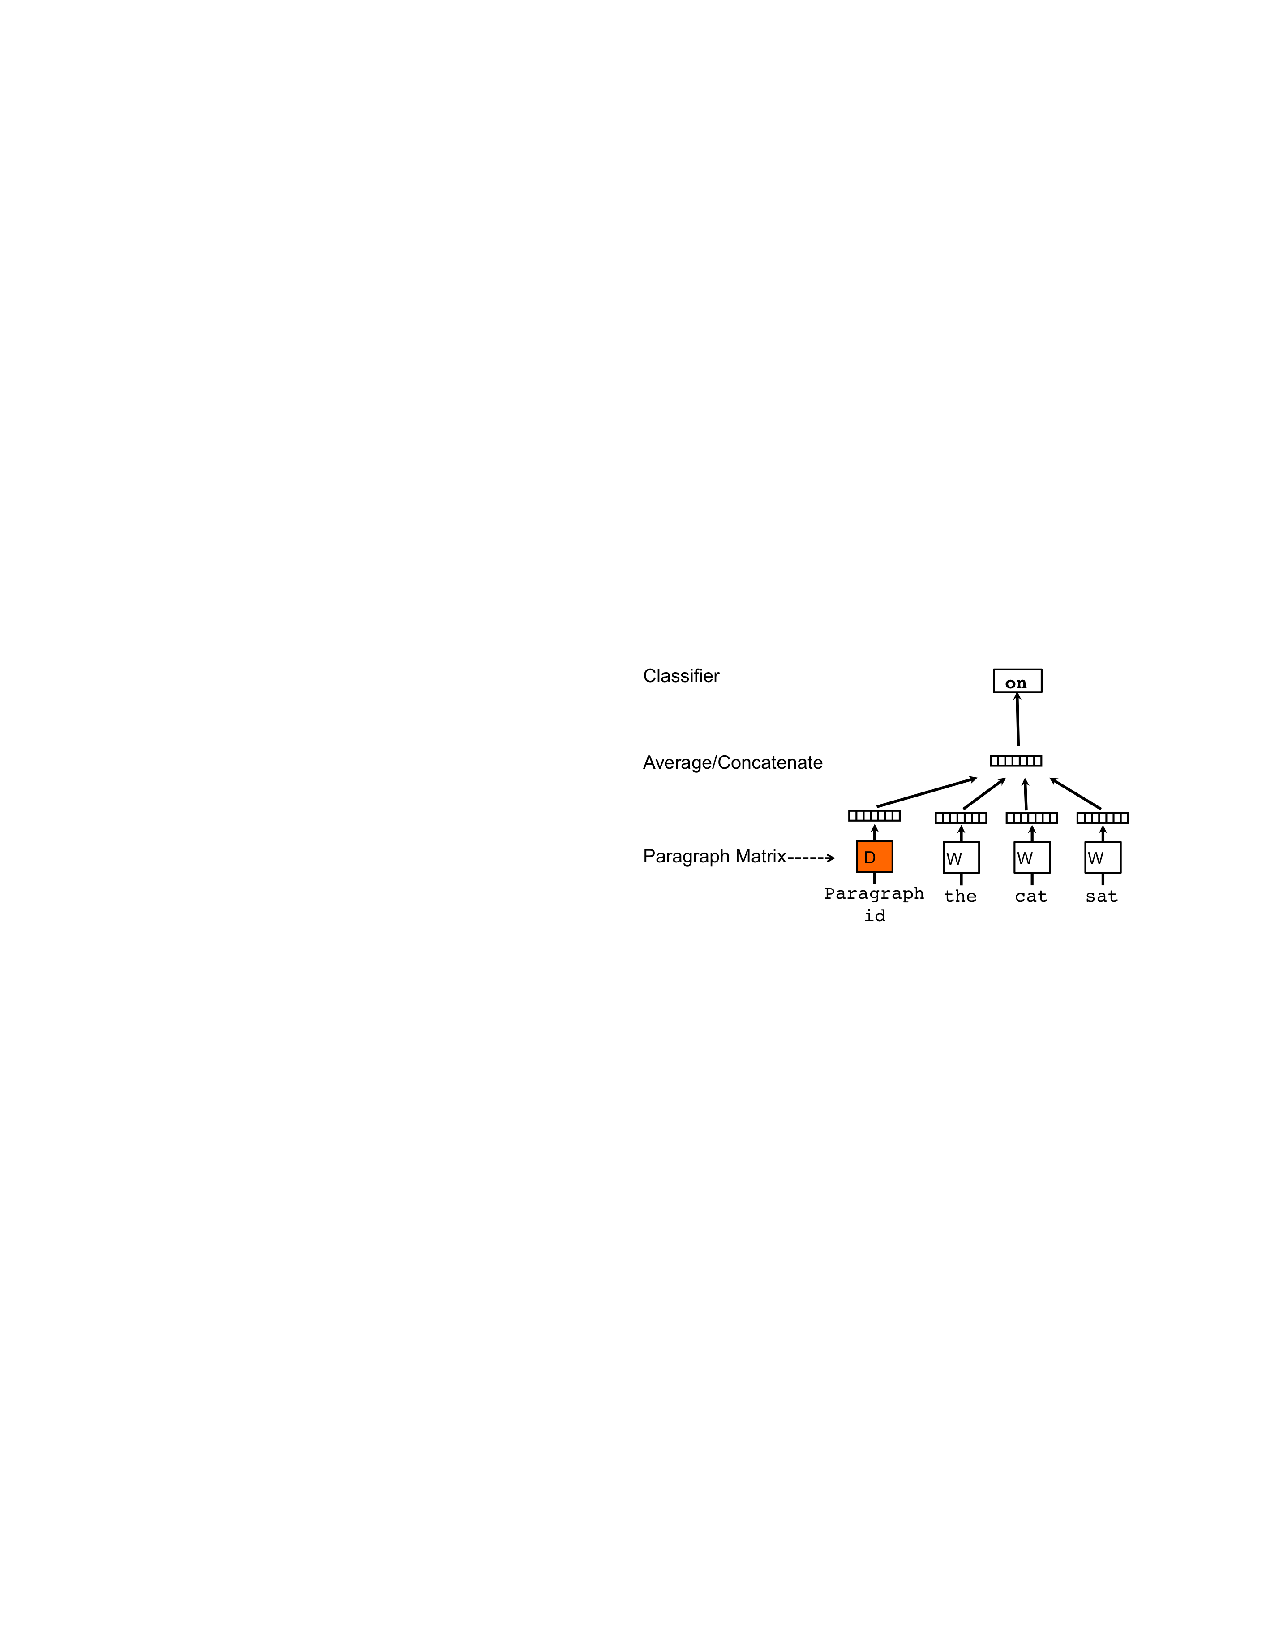
\includegraphics[width=0.5\columnwidth]{figures/methods/PV-DM}
\caption{The distributed memory model for paragraph vector.}
\label{fig:methods:PV-DM}
\end{figure}

In the previous section, we introduced one of the two models in word2vec, skip-gram. In skip-gram, one single word is used to predict every other word in the sentence, so that through back-propagation, the semantics of all other words is embedded in the word representation, resulting in a semantic embedding. In PV-DM (distributed memory for paragraph vector), a similar idea is adopted - a single paragraph vector is used to predict every word in the paragraph, so it can capture the semantics of all the words. Concretely, the model is defined by the following network structure, as shown in Figure~\ref{fig:methods:PV-DM}:

\begin{itemize}
    \item Each word in the dictionary is mapped to a word vector which is shared across all the sentence, just like word2vec. We can use pre-trained word vectors and fix them when training the paragraph vectors, or we can train the two representations simultaneously.
    \item Each paragraph is mapped to a vector (not necessarily in the same space with the word vectors), which is then passed through a feed-forward neural network, followed by a softmax output layer, just like skip-gram.
    \item The network predicts each word in the paragraph, with an opitimization objective of the log-likelihood of the whole corpus.
\end{itemize}

The only difference from skip-gram is that the word vector used for prediction is replaced with a pargraph vector.

\subsubsection{PV-DBOW}

\begin{figure}
\centering
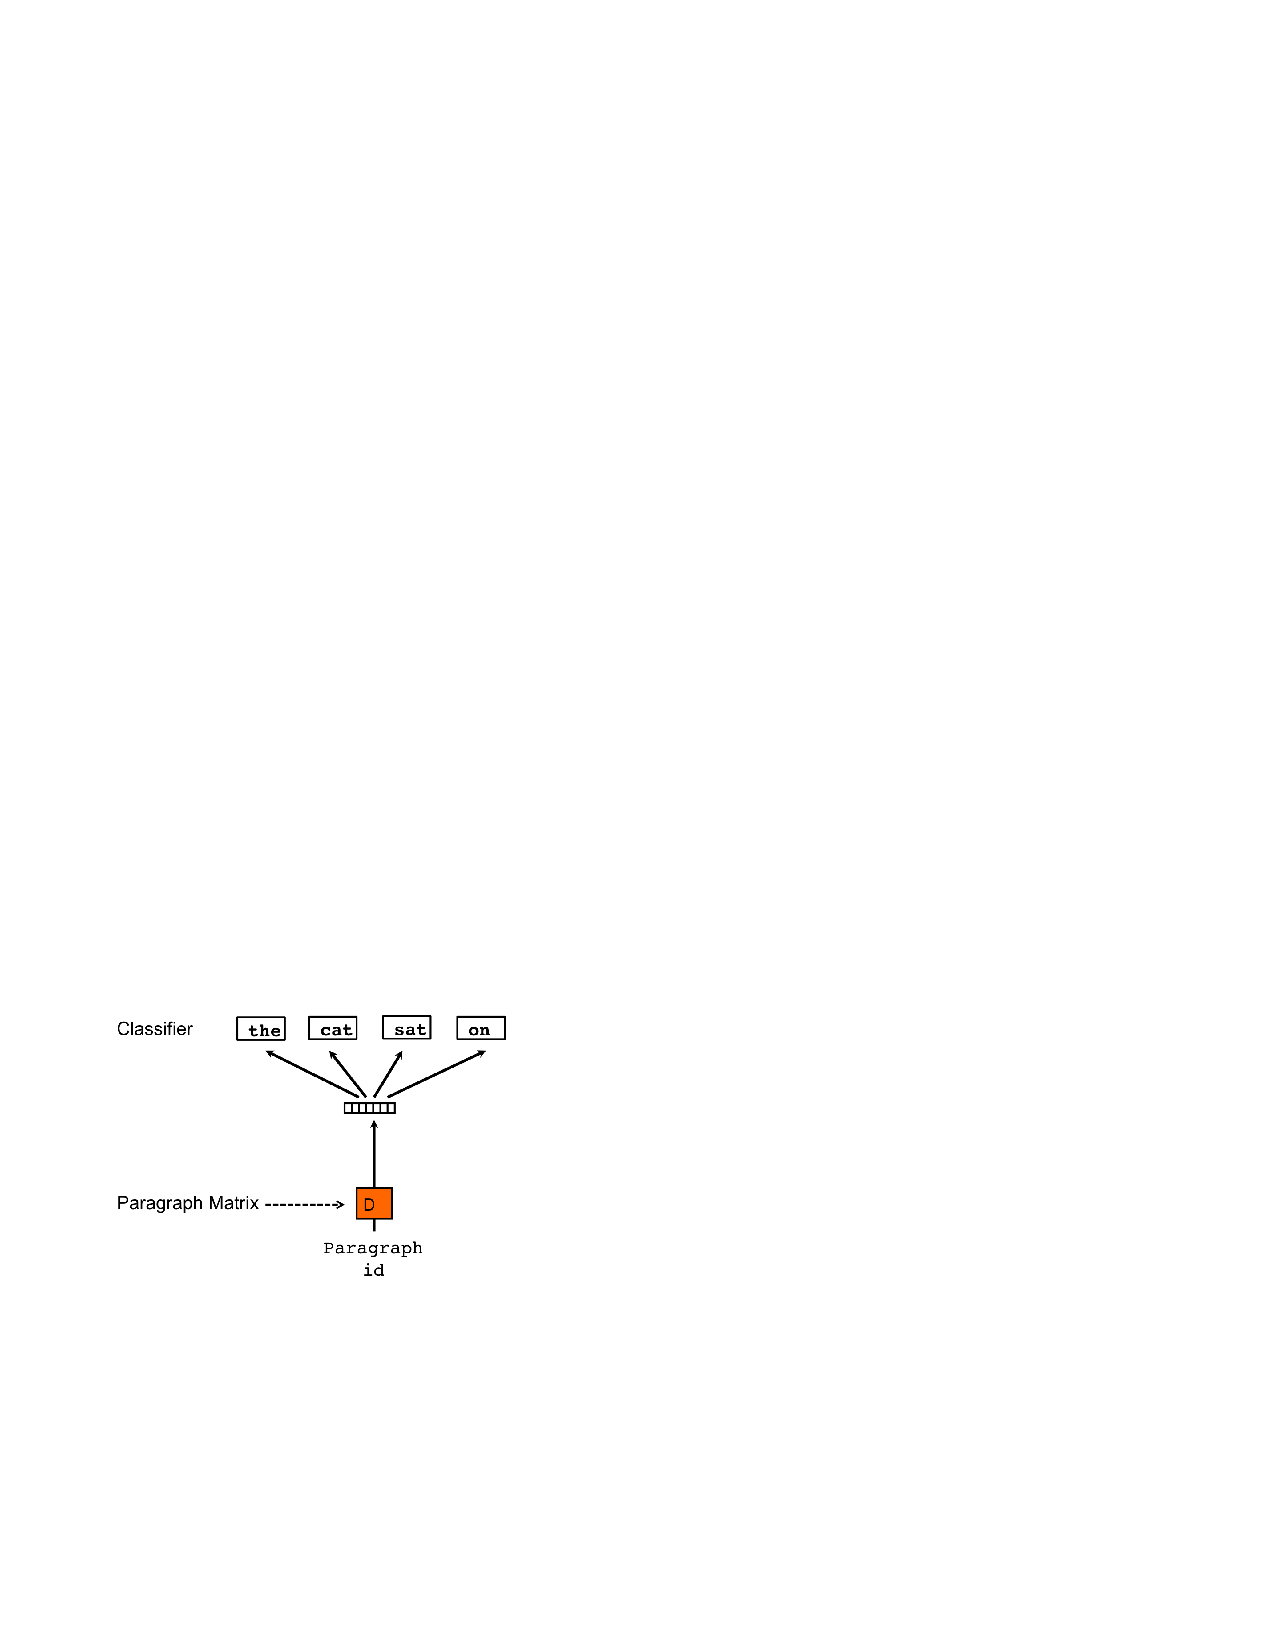
\includegraphics[width=0.5\columnwidth]{figures/methods/PV-DBOW}
\caption{The distributed bag-of-word model for paragraph vector.}
\label{fig:methods:PV-DBOW}
\end{figure}

PV-DBOW, or distributed bag-of-word for paragraph vector, is an extension to CBOW, continuous bag-of-word from word2vec. CBOW is defined by a n-gram neural network language model:

\begin{itemize}
    \item Each word is mapped to a vector.
    \item $n$ consecutive word vectors are concatenated together, fed through a feed-forward neural network and a softmax output layer to predict the next word in the sequence.
    \item The objective is the log-likelihodd of the whole corpus.
\end{itemize}

DBOW extends CBOW by using an extra paragraph vector, that is, in addition to the $n$ word vectors that are used to predict the next word, there is also a vector that represents the whole sentence, all concatenated together.The structure of PV-DBOW is shown in Figure~\ref{fig:methods:PV-DBOW}.

The final paragraph vector is the concatenation of the two vectors learned from PV-DM and PV-DBOW repectively and seperately.

\subsubsection{Advantages}

An important advantage of paragraph vector models is that they require no labeled data. Also, it doesn't require human experts to assign weights for words in a paragraph based on linguistic knowledge. The learned vector representations inherit an important property of word2vec, that is the semantics similarity. Also the final paragraph vector captures the word order information with the part learned from PV-DBOW with the n-gram model.

An advantage of paragraph vector over RNNs in practice is that it can leverage trained word vectors. The word vectors can be trained on a much larger corpus so they capture the semantics relationships more accurately, then the paragraph vecotrs can be trained on a relatively small dataset. Paragraph vectors are reported to word well with pre-trained word vectors. However, people find that it is more suitable to train the word vectors simultaneuosly for RNNs, so RNNs cannot leverage the word vectors learned from a larger dataset. Also, the paragraph vector models are simple and don't require storing a lot of information, by comparison for RNN we need to store every state during the forward pass for back-propagation, which is very memory consuming.
